%%%%%%%%%%%%%%%%%%%%%%%%%%%%%%%%%%%%%%%%%%%%%%%%%%%%%%%%%%%%%%%%%%%%%%%%%%%%
% AGUtmpl.tex: this template file is for articles formatted with LaTeX2e,
% Modified March 7, 2008, 3:30pm

\documentclass[wrr]{agutex}  %galley draft

\bibliographystyle{agufull04}

% LINE NUMBERS
% \usepackage{lineno}
% \linenumbers*[1]

  \usepackage{graphicx}
  \usepackage{tikz}
  \usetikzlibrary{shapes,arrows}
  \usetikzlibrary{shapes.symbols}
  \usetikzlibrary{backgrounds}
  

%    Allow illustrations to print when using Draft:
 \setkeys{Gin}{draft=false}
 \usepackage{subfigure,epstopdf}
 \usepackage{amsmath,amssymb}
 \usepackage[T1]{fontenc}
 \usepackage{fourier}
 \usepackage{palatino}
 \usepackage[scaled=.95]{couriers}
 \usepackage{booktabs}
 \newcommand{\p}{\partial}


%% ------------------------------------------------------------------------ %%
%  ENTER PREAMBLE
%% ------------------------------------------------------------------------ %%

% Author names in capital letters:
\authorrunninghead{BRACKEN}

% Shorter version of title entered in capital letters:
\titlerunninghead{ADAPTIVE MESHING AND SPARSE MATRIX STORAGE FOR STOKES FLOW}

% Author address will appear at end of article, please repeat
% this command for each author:

\authoraddr{C. W. Bracken,
Environmental Resources Engineering, Humboldt State University, Arcata, CA, USA.
(cwb12@humboldt.edu)}

\begin{document}

%% ------------------------------------------------------------------------ %%
%
%  TITLE
%
%% ------------------------------------------------------------------------ %%


\title{Unstructured adaptive mesh generation and sparse matrix storage applied to Stokes flow around cylinders}

%% ------------------------------------------------------------------------ %%
%
%  AUTHORS AND AFFILIATIONS
%
%% ------------------------------------------------------------------------ %%

\author{Cameron Bracken}
\affil{Environmental Resources Engineering, Humboldt State University, Arcata, CA, USA.}


%% ------------------------------------------------------------------------ %%
%
%  ABSTRACT
%
%% ------------------------------------------------------------------------ %%

% >> Do NOT include any \begin...\end commands within
% >> the body of the abstract.

\begin{abstract}
The flow field around cylindrical obstructions is computed by solving the Stokes equations.  An $h$-Method adaptive meshing algorithm is developed using a heuristic error indicator.  Pressure tended to produce the meshes with the lowest relative error in the least number of refinements.  SPARSE 
\end{abstract}

%% ------------------------------------------------------------------------ %%
%
%  BEGIN ARTICLE
%
%% ------------------------------------------------------------------------ %%

% The body of the article must start with a \begin{article} command
%
% \end{article} must follow the references section, before the figures
%  and tables.

\begin{article}

%% ------------------------------------------------------------------------ %%
%
%  TEXT
%
%% ------------------------------------------------------------------------ %%

\section{Introduction}
The Naiver-Stokes (NS) Equations are a set of vector valued nonlinear Partial Differential Equations (PDE's) which can be applied to any flowing fluid.  Common applications for the NS equations include ocean currents, weather, river hydraulics and airplane flight \citep{Chung2002}.  The Clay Mathematical Institute lists the theory relating to the NS equations as one of the seven most important outstanding problems in modern mathematics \citep{Clay2000}.  The NS equations are the cornerstone of a field known as Computational Fluid Dynamics (CFD).  The equations themselves represent conservation of momentum principals applied to a control volume.    The solution to the NS equations with a given set of boundary conditions are a set of functions $({\mathbf v}({\mathbf x},t), \rho({\mathbf x},t), p({\mathbf x},t))$, where ${\mathbf v}$ is the velocity field, $\rho$ is the density field and $p$ is the pressure field.

The linear form of the Navier-Stokes equations are called the Stokes equations.  These  equations are typically only applicable under extremely low Reynolds numbers ($Re<10$), also known as creeping flow.  These conditions may involve high fluid viscosities or low velocities or a combination of both 

Mesh generation is fundamental to numerical solutions of PDE's via the Finite Element (FE) method.  Node placement and mesh creation is often more of an art than a science, if not an arbitrary decision of the modeler.  Adaptive meshing techniques, a subset of multigrid methods, allow for efficient generation of ``optimal meshes.''  Adaptive mesh generation, while diverse in form, serves to negate the issue of manual node placement, manual mesh creation and global mesh refinement.  

The issue of mesh generation comes hand in hand with the issue of efficient solutions of the resulting system of equations.  The complete solution to the flow equations with a general mesh is computationally intensive if solved via direct methods.  In general the resulting matrices are spares and a large time and memory savings may be achieved by exploiting sparse matrix storage and solution methods.


%%%%%%%%%%%%%%%%%%%%%%%%%
\section{Problem Formulation}
We seek to solve the steady Stokes equations in 2D with cylindrical obstructions using an adaptively generated finite element (FE) mesh.  The stokes equations are solved via the FE method.  The unknowns of interest are velocity and pressure, $(\mathbf{v}(x,y),p(x,y))$.  Integrations are done in global coordinates via 3 point Gaussian quadrature.  The freely available software {\tt Triangle} is used to generate meshes given a set of nodes \citep{Shewchuk1996}.  The adaptive meshing algorithm uses an unstructured, h-adaptive, one-way refinement scheme based on a heuristic error indicator \citep{Bangerth2003}.  One-way refers to the fact that the algorithm only refines and does not derefine.  Average relative error of each method is compared.

The Stokes simulation model utilizes sparse matrix storage storage for the coefficient matrix $A$.  The corresponding system of linear equations is solved using sparse matrix library {\tt SLAP} \citep{Anderson1999} as well as the dense matrix library {\tt LAPACK}.  Solution times using both sparse and dense solvers are compared.  
 
%%%%%%%%%%%%%%%%%%%%%%%%% 
\section{Literature Review}
 
The CFD has historically been dominated by the finite difference (FD) method \citep{Chung2002}.  FD methods tend to have much simpler formulations and be less computationally intensive but they do not support unstructured grids.  One of the earliest applications of the FD method in CFD was \cite{Courant1928}.  

FE formulations require more mathematical rigor than FD methods but they support unstructured meshes and irregular problem domains.  FE work was first published by \cite{Turner1956}.  2D flow past a cylinder is a common application of the Stokes equations \citep{Bangerth2003}.  One aim in modeling flow around a cylinder is to calculate the drag coefficient. 

\subsection{Grid Generation}
There are two main types of FE grid generation, 
\begin{enumerate} 
\item {\it Structured Grid generation} involves some pattern of isoparametric elements which exploit the geometry of a problem domain for efficient mesh generation.  Structured grid generation may need to be preformed piecewise for complex geometries.  Structured grids apply only in 2 and 3D.
\item {\it Unstructured Grid generation} involves the use of Delaunay-Voronoi triangulation of a set of points.  Many algorithms for constrained of Delaunay triangulation exist including the Watson algorithm \cite{Watson1981} and {\tt Triangle} \citep{Shewchuk1996}.
\end{enumerate}

\subsection{Adaptive Meshing}
Adaptive meshing techniques can apply to structured or unstructured mesh generation in 1, 2, or 3D.  Let $E_e$ be an estimate of the actual error $\mathcal{E}_e$ error for element $e$.  Adaptive meshing is used to refine or unrefine (coarsen) meshes based on $E_e$, (usually based on the solution gradient)\citep{Chung2002}.  $E_e$ is called an a priori error estimate because they require a precomputed solution in order to be calculated.  The focus here will be in unstructured adaptive methods. There are three main methodologies in unstructured mesh refinement
\begin{enumerate} 
\item {\it h-Methods} also known as mesh refinement methods, refine elements which have a high a priori error by adding nodes and vertices.  
\item {\it r-Methods} also known as mesh movement methods, do not add any new nodes but simply move existing nodes in order to obtain the lowest possible global error.  
\item {\it p-Methods} also known as mesh enrichment methods, increase the degree of the polynomial interpolating function for a particular element with high a priori error estimate. 
\end{enumerate}
Additionally many hybrid methods exist which combine the ideas from the three basic adaptive mesh methods.  Some of these hybrid methods are combined mesh refinement and mesh movement ({\it hr}-methods) and combined mesh refinement and mesh enrichment ({\it hp}-methods). 

For all unstructured adaptive mesh techniques, the general procedure involved is

\begin{enumerate}
\item Solve the  simulation model.
\item Obtain an estimate of the local relative error over each element using some error indicator (typically $u$, $v$, $p$ or $\rho$ in a CFD problem).
\item Identify elements with high relative error.
\item Somehow increasing the accuracy of the solution over elements which have high error and 
\item Repeating until a global error tolerance is met.
\end{enumerate}

\subsection{Sparse Matrix Storage and Computation} \label{sec:sparse}
In 1D coefficient matrices resulting from the FE method are tightly banded and may be stored and solved efficiently.  For structured meshes in 2D coefficient matrices are typically banded and thus banded storage and solution algorithms can be used with savings over dense solvers \citep{Burkardt2005c}.  For unstructured meshes in 2D coefficient matrices are typically sparse and unbanded.  The sparsity is especially pronounced for adaptively generated meshes. Thus, general sparse matrix storage and computation is crucial for efficient solutions to large problems.  

Sparse matrix data structures come in many forms all of which attempt to only store nonzero entries of a sparse matrix.  The most simple storage structure is called the coordinate format or the Triad format \citep{Anderson1999} which stores the row number, column number and nonzero entries in vectors of equal length.  Other, more efficient storage structures include the compressed sparse row format, compressed sparse column format, and the sparse block storage format.  The coordinate format is used in this paper.  

If we let $n_s$ be the number of nonzero entries in the matrix A of dimension $N$, then the coordinate format will only provide storage savings if $3n_s<N^2$.  Dense matrix storage increases as $N^2$ where sparse storage increases linearly with $N$.

 
%%%%%%%%%%%%%%%%%%%%%%%%%
\section{Model Formulation and Development}
This section will address the simplification of the Navier-Stokes equations, finite element formulation, quadrature rule over the general triangle and the adaptive meshing algorithm.  
\subsection{Navier-Stokes Simplification}
The NS Equations for unsteady compressible flow are 

\begin{equation}
  \rho {\bf v}_t - \mu \nabla^2 {\bf V} + \rho ({\bf V}  \cdot \nabla ) {\bf v} 
    + \nabla p = 0 \label{eqn:ns}
\end{equation}
where $\mu$ is the kinematic viscosity \citep{Chung2002}.  The NS equations are typically coupled with the continuity equation for fluids

\begin{equation}
\rho_t + \nabla \cdot (\rho \mathbf{V}) = 0.
\end{equation}

If we assume that the flow is steady, incompressible and uniform in the $z$ direction then $\mathbf{V}(\mathbf{x},t) = \mathbf{V}(x,y) = (u(x,y),v(x,y))$.  If we further construct a situation involving very low Reynolds number ($Re<10$), the nonlinear term in equation \ref{eqn:ns} will be small resulting in the Stokes equations 

\begin{equation}
  - \mu \nabla^2 {\bf V} + \nabla p = 0 \label{eqn:momentum}
\end{equation}
and the associated continuity equation

\begin{equation}
\nabla \cdot \mathbf{V} = 0. \label{eqn:continuity}
\end{equation}

The Stokes equations are linear and the solution is the set of functions $({\mathbf V}(x,y), p(x,y))$.

\subsection{Finite Element Formulation}\label{sec:fe_devel}
We begin by constructing a piecewise approximate solution to the Stokes equation $\hat{\mathbf{V}}(x,y)$ and $\hat{p}(x,y)$ where 
\begin{equation}
\mathbf{V}(x,y)\approx\hat{\mathbf{V}}(x,y)=\sum_{j=1}^{n_v}\phi_j(x,y)\tilde{\mathbf{V}}_j
\end{equation}
\begin{equation}
p(x,y)\approx\hat{p}(x,y)=\sum_{j=1}^{n_p}\psi_j(x,y)\tilde{p}_j
\end{equation}
where $\phi_i(x,y)$ and $\psi_i(x,y)$ are the interpolating functions associated with velocity and pressure respectively, $\tilde{\mathbf{V}}_j$ and $\tilde{p}_j$ are the nodal values velocity and pressure, $n_v$ is the number of velocity nodes and $n_p$ is the number of pressure nodes.  This formulation allows us to have a different number of velocity and pressure nodes.  From this point on the explicit dependency in $x$ and $y$ will be dropped in the interest concision.  

The necessary conditions of the FE method, which minimize global error of the approximate solution, are 

\begin{equation}
\int_\Omega \mathbf{w}_i\mathcal{L}\{\hat{\mathbf{V}},\hat{p}\}\,\,\,d\Omega= 0 \label{eqn:galerkin}
\end{equation}
where $\Omega$ is the problem domain, $\mathbf{w}_i$ are weighting functions and $\mathcal{L}$ is the Stokes operator given by equations \ref{eqn:momentum} and \ref{eqn:continuity} \citep{Willis1987}.  The Galerkin method sets the weighting functions equal to the interpolating functions such that $\mathbf{w}_i = (\phi_i,\psi_i)$.  The equations so far are not very useful to us, but if we apply the stokes operator and multiply by the weighting functions we start to formulate the useful FE equations

\begin{equation}
\int_\Omega\phi_i(\nu \nabla^2 \hat{{\mathbf V}} + \nabla \hat{p})\,\,\,d\Omega= 0 
\end{equation}

\begin{equation}
\int_\Omega\psi_i\nabla \cdot \hat{\mathbf{V}}\,\,\,d\Omega= 0 .
\end{equation}
which are known as the strong form of the Stokes equations.  A solution to these equations is a so called strong solution. A strong solution, due to the second derivative term, requires the interpolating functions be at least $C^2(\Omega)$ functions \citep{Burkardt2005c}.

We can derive the weak form of the Stokes equations via integration by parts, which states that for a continuously differential functions $B$ and $\mathbf{F}$ defined over some region $\Omega$

\begin{equation}
  \iint_\Omega B\nabla^2\mathbf{F}\,\,\,d\Omega = -\iint_\Omega \nabla B \nabla \mathbf{F}\,\,\,d\Omega+\oint_{\partial\Omega}B\nabla \mathbf{F}\cdot\mathbf{n} \,\,\,ds.
\end{equation}
where $B$ is a general function and $\mathbf{F}$ is a vector valued function both defined on $\Omega$ and $\mathbf{n}$ is an outward pointing unit normal vector on $\p\Omega$ \citep{Marsden2003}.

Letting $B=\phi_i$ and $\mathbf{F}=\hat{\mathbf{V}}$

\begin{equation}
  \iint_A \nu \nabla\phi_i\cdot \nabla \hat{\mathbf{V}} 
  + \phi_i\nabla p\,\,\,dA  = \oint_s\phi_i\nabla \hat{\mathbf{V}} \,\,\,ds.
  \label{eqn:weak1}
\end{equation}
%
\begin{equation}
  \iint_A\psi_i\nabla \cdot \hat{\mathbf{V}}\,\,\,dA = 0
  \label{eqn:weak2}
\end{equation}

which are known as the weak form of the Stokes equations.  The solution to these equations are only required to be $C^1(\Omega)$ functions which will simplify the solution process and allow us to use linear basis functions \cite{Burkardt2005b}.  

Let us examine equation \ref{eqn:weak1} in order to explicitly formulate the equations associated with the weak Stokes equations.  There are $2n_v+n_p$ linear equations associated with these equations \ref{eqn:weak1} and \ref{eqn:weak2} because equation \ref{eqn:weak1} is vector valued with two components. Substitute in the piecewise approximate solutions $\hat{\mathbf{V}}$ and $\hat{p}$ into the left hand side of equation \ref{eqn:weak1}

$$
  \iint_A \nu \nabla \phi_i \nabla\sum_{j=1}^{n_v}\phi_j\tilde{\mathbf{V}}_j
  + \phi_i\nabla\sum_{j=1}^{n_p}\psi_j\tilde{p}_j\,\,\,dA  = \oint_{\partial A}\phi_i\nabla \hat{\mathbf{V}}_j \,\,\,ds 
$$

\begin{multline}
  \iint_A \nu \sum_{j=1}^{n_v}\nabla \phi_i\nabla\phi_j\tilde{\mathbf{V}}_j
  + \sum_{j=1}^{n_p}\phi_i\nabla\psi_j\tilde{p}_j\,\,\,dA  =\\ \oint_{\partial A}\phi_i\nabla \hat{\mathbf{V}}_j \,\,\,ds \label{eqn:full1}
\end{multline}
Analogously for equation \ref{eqn:weak2} we can write

\begin{equation}
\iint_A\sum_{j=1}^{n_v}\tilde{\mathbf{V}}_j\psi_j\nabla\phi_i\,\,\,dA = 0 \label{eqn:full2}
\end{equation}

Using equations \ref{eqn:full1} and \ref{eqn:full2} we can formulate a system of linear equations with dimension $2n_v+n_p$ of the form 

\begin{equation}
A\mathbf{g}+\mathbf{f} = 0
\end{equation}
where $\mathbf{g}=[\tilde{\mathbf{u}}\,\,\,\,\tilde{\mathbf{v}}\,\,\,\,\tilde{\mathbf{p}}]^T$ and T denotes transpose.  It is useful to note here that the $A_{ij}$ coefficient of $\mathbf{V}_j$ is 

$$\left[\iint_A\nabla \phi_i\cdot\nabla\phi_j\,\,\,dA+\iint_A\nabla\psi_j\phi_i\,\,\,dA\right]$$ 
and of $p_j$ is 

$$\left[\iint_A\phi_i\nabla \psi_j\,\,\,dA\right]$$ 

An algorithm to assemble the stokes equations must take into account that $\phi_i$ and $\psi_i$ need not be defined at the same nodes.  Also note that equation \ref{eqn:full1} is vector valued.  The scalar versions will be presented in Section \ref{model_application}. 

%%%%%%%%%%%%%%%%%%%%%%%%%%%%%%%%%%%%%%%
\subsection{Adaptive Meshing Algorithm}
The required components of an $h$ adaptive mesh refinement scheme are an error indicator, an error estimate and a refinement procedure.  Let $\theta_n$ be the error indicator for every node $n$ and $E_e$ be the a priori error estimate for element $e$.  In the stokes problem $\theta_n$ may be horizontal velocity, vertical velocity or pressure.  We define the relative percent error, $E_e$ for an element with verticies $(i,j,k)$ as

\begin{equation}
E_e = {\left[\max\left(\theta_i,\theta_j,\theta_k\right)-\min\left(\theta_i,\theta_j,\theta_k\right)\right] \left\|\underline{\theta}\right\|^{-1}}\label{eqn:err}
\end{equation}
This relative error estimate is is known as a heuristic type error estimte\citep{Bangerth2003}.  There exist many other error estimation methods which will not be discussed in this paper.  

If we take $E_e$ to be a surrogate for the actual error and $h_e$ to be a element length scale then the assumption is that as $h_e\rightarrow 0$,$E_e\rightarrow 0$.  Therefore we introduce the parameters $A_{min}$, the minimum allowable element area, $\epsilon$, the maximum allowable relative percent error, and $m$ the maximum allowable number of elements that do not meet the error or area criteria.  The algorithm for one way adaptive meshing is 

\begin{enumerate}
\item Generate an initial sparse set of points.
\item Generate mesh.
\item Solve Stokes equations to determine $I_e$.
\item Evaluate $E_e$ and $A_e$for all elements $e$ using equation \ref{eqn:err}.
\item For all elements e
	\begin{enumerate}
		\item IF $E_e>\epsilon$ and $A_e>A_{min}$, mark element $e$ for refinment
		\item ELSEIF do not mark element $e$ for refinement.  
	\end{enumerate}
\item IF number of elements to refine is $<m$ FINISH.
\item ELSE Refine elements marked for refinement by placing a new node at the center of the element.
\item GO TO step 2.
\end{enumerate}

\begin{figure}
\centering
%\noindent\includegraphics[width=13pc]{figs/flochart.pdf}
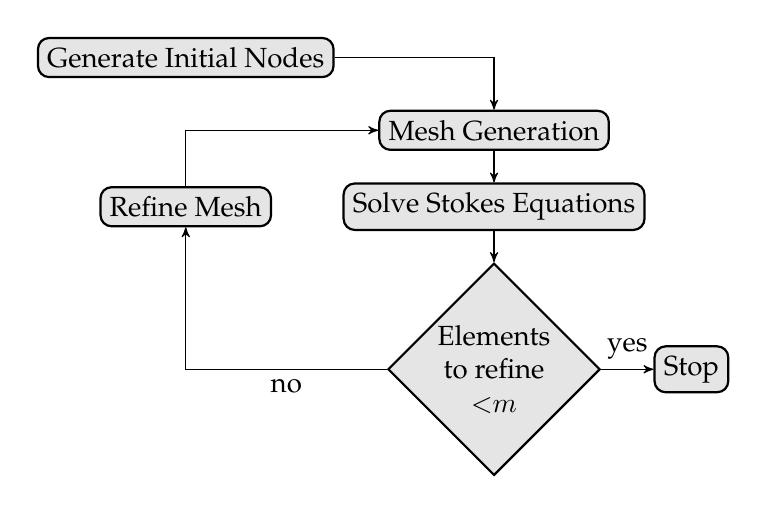
\begin{tikzpicture}
[ auto,
decision/.style={diamond, draw=black, thick, fill=gray!20, 
text width=4.5em, text badly centered, 
inner sep=0pt}, 
block/.style ={rectangle, draw=black, thick, fill=gray!20, 
 text centered, rounded corners, 
%text width=5em,minimum height=4em
}, ] 
\matrix [column sep=1mm,row sep=4mm] 
{ 
% row 1 
%\node (expert) [cloud] {expert}; & 
\node (init) [block] {Generate Initial Nodes}; 
%\node (system) [cloud] {system}; 
\\ 
% row 2 
& \node(identify) [block] {Mesh Generation};  \\ 
% row 3 
\node (update) [block] {Refine Mesh}; & 
\node (evaluate)[block] {Solve Stokes Equations};  \\ 
% row 4 
& \node (decide)[decision] {Elements to refine $<$$m$};  
& \node (stop)[block] {Stop};  \\ 
}; 

\draw[-stealth'] (init) -| (identify); 
\draw[-stealth'] (identify) -- (evaluate); 
\draw[-stealth'] (evaluate) -- (decide); 
\draw[-stealth'] (update) |- (identify); 
\draw[-stealth'] (decide) -| node [near start] {no} (update); 
\draw[-stealth'] (decide) -- node [midway] {yes} (stop); 
%\draw[-stealth'] [dashed] (expert) -- (init); 
%\draw[-stealth'] [dashed] (system) -- (init); 
%\draw[-stealth'] [dashed] (system) |- (evaluate); 
\end{tikzpicture} 
\caption{Mesh refinement algorithm flowchart.}
\end{figure}



\section{Model Application}\label{model_application}
This section gives a formal statement of the problem in question, discusses basis functions and quadrature, defines parameter values, discusses the software used and the programming framework. 
	
\subsection{Formal Problem Statement}
The Stokes equations in scalar form are 
	\begin{equation}
  - \nu \frac{\p^2 u}{\p x^2} 
  - \nu \frac{\p^2 u}{\p y^2} 
%  + u \frac{\partial u}{\partial x} + v \frac{\partial u}{\partial y} 
  + \frac{\p p}{\p x}  = 0 
\label{eqn-h-mom}
\end{equation}
%
\begin{equation}
  - \nu \frac{\p^2 v}{\p x^2} 
  - \nu \frac{\p^2 v}{\p y^2}
%  +  u \frac{\partial v}{\partial x} + v \frac{\partial v}{\partial y} 
  + \frac{\p p}{\p y}  = 0 
\label{eqn-v-mom}
\end{equation}
%
\begin{equation}
  \frac{\p u}{\p x} + \frac{\p v}{\p y} = 0
\label{eqn-cont}
%
\end{equation}

With the associated set of boundary conditions:
\begin{equation}0\leq x\leq L_x ,\,\,\,0\leq y\leq L_y\end{equation}
\begin{equation}v(x,0)=k\,x\,(1-x),\,\,\,u(x,0)=0\end{equation}
\begin{equation}\left.\frac{\partial \mathbf{v}}{\p x}\right|_{(x,L_y)}=0\end{equation}
\begin{equation}\mathbf{v}(0,y)=0,\,\,\,\mathbf{v}(L_x,y)=0\end{equation}
\begin{equation}p(x_o,y_o)=0\end{equation}
Inflow boundary conditions are a parabolic vertical velocity profile perpindicular to the boundary.  Outflow boundary conditions require that flow be perpendicular to the boundary. The left and right side and obstruction boundary conditions are no slip (zero Dirchlet).  Pressure is a potential function and thus need only to be specified at a single point $(x_p,y_p)$

\begin{figure}[h]
\begin{center}
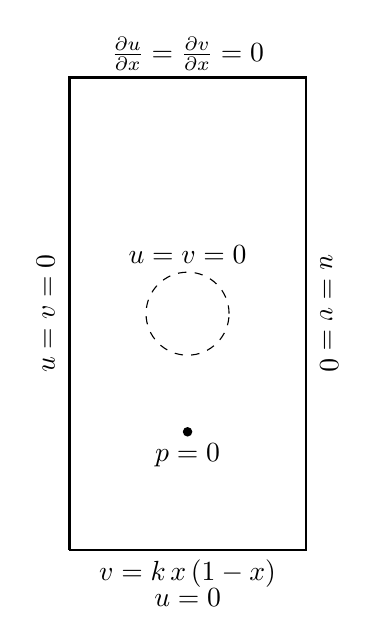
\begin{tikzpicture}[scale=3]
	\draw[thick](0,0)--(0,2)--(1,2)--(1,0)--(0,0);
	
	\draw (.5,2.1) node{${\p u\over\p x}={\p v\over\p x}=0$};
	\draw (.5,-.1) node{$v=k\,x\,(1-x)$};
	\draw (.5,-.2) node{$u=0$};
	\draw (-.1,1) node[rotate=90]{$u=v=0$};
	\draw (1.1,1) node[rotate=-90]{$u=v=0$};
	\draw[style=dashed] (.5,1) circle(5pt);
	\draw (.5,1.25) node{$u=v=0$};
	\filldraw [black] 
		(.5,.5) circle (.5pt);
	\draw (.5,.4) node{$p=0$};
	
\end{tikzpicture}
\end{center}
\caption{Problem domain with cylindrical obstruction which may or may not be present.}\label{fig:tri}
\end{figure}

The FE formulation written in scalar form for any internal node 
\begin{equation}
  \iint_A \nu \sum_{j=1}^{n_v}\left\{{\p\phi_i\over\p x}{\p\phi_j\over\p x}+{\p \phi_i\over\p y}{\p\phi_j\over\p y}\right\}\tilde{u}_j
  + \sum_{j=1}^{n_p}\phi_i\frac{\p \psi_j}{\p x}\tilde{p}_j\,\,\,dA  = 0\label{eqn:full222}
\end{equation}
\begin{equation}
  \iint_A \nu \sum_{j=1}^{n_v}\left\{{\p\phi_i\over\p x}{\p\phi_j\over\p x}+{\p \phi_i\over\p y}{\p\phi_j\over\p y}\right\}\tilde{v}_j
  + \sum_{j=1}^{n_p}\phi_i\frac{\p \psi_j}{\p y}\tilde{p}_j\,\,\,dA  = 0\label{eqn:full222}
\end{equation}

\begin{equation}
\iint_A\sum_{j=1}^{n_v}\left\{u_j\frac{\p \psi_j}{\p x}+v_j{\p \psi_j \over \p y}\right\}\phi_i\,\,\,dA = 0 \label{eqn:full3333}
\end{equation}

%%%%%%%%%%%%%%%%%%%%%%%%%%%%%%%%
\subsection{Basis Functions}

In this section we use the terms interpolating function and basis function interchangeably. We saw in section \ref{sec:fe_devel} that we need two basis functions, $\psi_i$ and $\phi_i$, one for the momentum equation and one for the continuity equation.  For this problem we will use Taylor-hood elements.  These elements use linear basis functions for pressure and quadratic basis functions for a single element. Figure \ref{fig:tri} shows an archetypal linear pressure element with nodes defined at the vertices. Figure \ref{fig:tri2} shows an archetypal quadratic velocity element with nodes defined at the vertices as well as at the midside of the vertices.

The linear basis functions for pressure as given in \cite{Lapidus1982} is 

\begin{equation}
  \psi_i(x,y) = \frac{ ( x   - x_j )  ( y_k - y_j ) - ( x_k - x_j )  ( y   - y_j ) }
                     { ( x_i - x_j )  ( y_k - y_j ) - ( x_k - x_j )  ( y_i - y_j ) }
\end{equation}

Quadratic basis functions for a triangle are derived inas given in \cite{Burkardt2005b}; here we will state them without proof. For the three vertex nodes
\begin{equation}
  \phi_i(x,y) = \frac{ g_v(x,y) \, h_v(x,y) } {  g_v(x_i,y_i) \, h_v(x_i,y_i)  }
\end{equation}
where 
\begin{equation}
  g_v(x,y) = ( x - x_j ) ( y_k - y_j ) - ( x_k - x_j ) ( y - y_j )
\end{equation}
and
\begin{equation}
  h_v(x,y) = ( x - x_{ij} ) ( y_{ik} - y_{ij} ) - ( x_{ik} - x_{ij} ) ( y - y_{ij} )
\end{equation}
where $(x_{ij},y_{ij})$ is the coordinate associated with the midside node between nodes $i$ and $j$.

As given in \cite{Burkardt2005b}, the basis functions associated with the midside nodes are
\begin{equation}
  \psi_{ij}(x,y) = \frac{ g_m(x,y) \, h_m(x,y) }{ ( g_m(x_{ij} ,y_{ij} ) \, h_m(x_{ij} ,y_{ij} ) }
\end{equation}
where
\begin{equation}
  g_m(x,y) = ( x - x_k ) ( y_i - y_k ) - ( x_i - x_k ) ( y - y_k )
\end{equation}
and
\begin{equation}
  h_m(x,y) = ( x - x_k ) ( y_j - y_k ) - ( x_j - x_k ) ( y - y_k ).
\end{equation}

It is interesting to note that
\begin{multline}
  \psi_i(x,y) + \psi_j(x,y) + \psi_k(x,y) + \psi_{ij}(x,y) 
  \\+ \psi_{jk}(x,y) + \psi_{kj}(x,y) = 1
\end{multline}
will hold true for any non-degenerate element.

\begin{figure}[h]
%\begin{center}
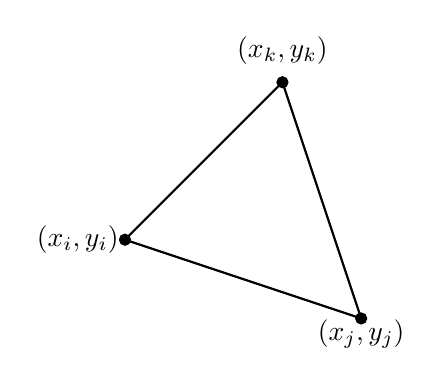
\begin{tikzpicture}[scale=2]
	\draw[thick](0,0)--(1,1)--(1.5,-.5)--(0,0);
	
	\filldraw [black] (0,0) circle (1pt) 
				(1,1) circle (1pt) 
				(1.5,-.5) circle (1pt);
				
	\draw (-.3,0) node{$(x_i,y_i)$};
	\draw (1.5,-.6) node{$(x_j,y_j)$};
	\draw (1,1.2) node{$(x_k,y_k)$};
	
\end{tikzpicture}
%\end{center}
\caption{Archetypal linear pressure element.}\label{fig:tri}
\end{figure}


\begin{figure}[h]
%\begin{center}
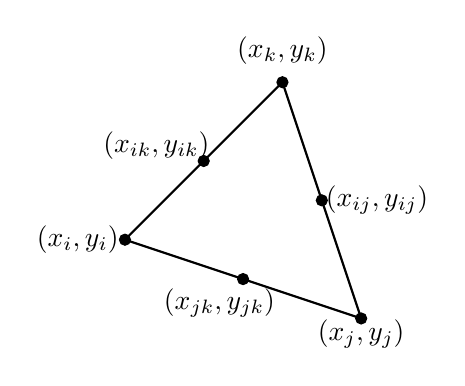
\begin{tikzpicture}[scale=2]
	\draw[thick]
		(0,0)--(1,1)--(1.5,-.5)--(0,0);
	
	\filldraw [black] 
		(0,0) circle (1pt) 
		(1,1) circle (1pt) 
		(1.5,-.5) circle (1pt)
		(.5,.5) circle (1pt) 
		(.75,-.25) circle (1pt) 
		(1.25,.25) circle (1pt);
				
	\draw 
		(-.3,0) node{$(x_i,y_i)$}
		(1.5,-.6) node{$(x_j,y_j)$}
		(1,1.2) node{$(x_k,y_k)$}
		(.2,.6) node{$(x_{ik},y_{ik})$}
		(.6,-.4) node{$(x_{jk},y_{jk})$}
		(1.6,.25) node{$(x_{ij},y_{ij})$};
	
\end{tikzpicture}
%\end{center}
\caption{Archetypal quadratic velocity element.}\label{fig:tri2}
\end{figure}

%%%%%%%%%%%%%%%%%%%%%%%%%%%%%%%%%%%%%%%%%%%%%%%%
\subsection{Quadriture Over a General Triangle}
The reference triangle $T_r$ has vertices (0,0), (0,1) and (1,0) in dimensionless coordinates $(\xi,\eta)$. Gaussian quadrature for the reference triangle is 
\begin{equation}
  \int_{T_r}f(\xi,\eta)\,\,\,d\xi d\eta=\sum_{p=1}^{n}w_pf(\xi_p,\eta_p).
\end{equation}
The values of $w_p,\xi_p$ and $\eta_p$ are tabulated in \cite{Lapidus1982}.  

Since our basis functions (and subsequent integrals) are defined in global coordinates, we need a way to map quadrature points and weights in the reference triangle to points in the actual triangle $T$.  The mapping is developed in \cite{Burkardt2005b}.  To map any point $(\xi_p,\eta_p)$ to a point $(x_p,y_p)$ in the triangle T we use 

\begin{equation}
  \left[\begin{array}{c} x_p \\ y_p \end{array} \right] = 
  \left[\begin{array}{c} x_i \\ y_i \end{array}\right] +
  \left[\begin{array}{cc} x_j-x_i & x_k-x_i \\ y_j-y_i & y_k-y_i\end{array}\right]
  \left[\begin{array}{c} \xi_p \\ \eta_p \end{array}\right]
\end{equation}
We can write our quadrature rule as 
\begin{equation}
  \int_{T}f(x,y)\,\,\,dxdy=A_T\sum_{p=1}^{n}w_pf(x_p,y_p).
\end{equation}
Where $A_T$ is the area of the triangle which is the artifact of a constant Jacobian for our linear mapping.  The area of the triangle is given by 
\begin{equation}
A_T=\left[\begin{array}{ccc}1 & x_i & y_i \\1 & x_j & y_j \\1 & x_k & y_k\end{array}\right]
\end{equation}


%%%%%%%%%%%%%%%%%%%%%%%%%%%%%%
\subsection{Software}
The software library {\tt SLAP} (Sparse Linear Algebra Package) \citep{Seager1988} is used to solve the linear system of equations.  {\tt SLAP} is a set of matrix algebra routines, written in {\tt Fortran 77} for large sparse linear systems and is available for free at {\tt netlib.org}. Specifically the routine {\tt DGMRES} is used where the coefficient matrix is stored in the {\tt SLAP} triad format.  The triad format identical to the coordinate format described in section \ref{sec:sparse}.  {\tt DGMRES} solves the linear system $Ax=b$ using the generalized minimum residual method \citep{Seager1988}.  

{\tt LAPACK} is an industry standard library of dense and banded solvers for systems of linear equations \citep{Anderson1999}.  {\tt LAPACK} has been optimized for many computer systems and is based on the {\tt BLAS} (Basic linear algebra subroutines) library.  Here we use the version of {\tt LAPACK} optimized by Apple computers as part of the {\tt Accelerate} framework.  The specific routine used is the {\tt DGETRS} which uses LU decomposition to factor the coefficient matrix.  
	
{\tt Triangle} is freely available software for creating 2D quality constrained meshes.  By quality we mean that the mesh generator will add vertices to the mesh where appropriate to ensure that a minimum angle requirement is met \citep{Shewchuk1996}.  {\tt Triangle} creates a conforming constrained Delaunay triangulation where each triangle in not necessarily Delaunay but that does not matter for a finite element mesh.  The software is written in {\tt C} and therefore difficult to interface directly with {\tt Fortran}.  This issue is circumvented by writing the program framework as a bash shell script which deals in I/O files. 

John Burkhardt created a Navier-Stokes simulation model called {\tt free\_fem\_navier\_stokes} from which some subroutines were used for this problem \citep{Burkardt2007}.  Specifically the subroutines for evaluating the basis functions and assembling the coefficient matrix.  

The initial node generation program is called {\tt regmeshgen}, the main simulation program is called {\tt stokes\_sim} the error analysis program is called {\tt adaptive} and the mesh refining program is called {\tt nodegen}.  A flowchart of the software framework is shown in figure \ref{fig:sf}.
 

\begin{figure}[h]
%\begin{center}
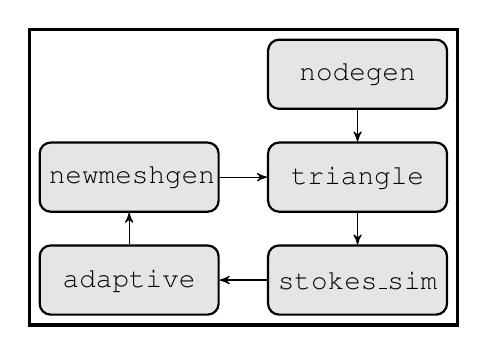
\begin{tikzpicture} 
[auto,  
block/.style ={rectangle, draw=black, thick, fill=gray!20, 
text width=5.8em, text centered, rounded corners, 
minimum height=2.5em}]

\matrix [column sep=6mm,row sep=4mm,draw,very thick ] 
{ 
% row 1 
%\node (expert) [cloud] {expert}; & 
&\node (init) [block] {{\tt nodegen}}; 
%\node (system) [cloud] {system}; 
\\ 
% row 2 
\node (new) [block] {{\tt newmeshgen}}; &
\node(tri) [block] {{\tt triangle}};  \\ 
% row 3  
\node (adaptive) [block] {{\tt adaptive}}; &
\node (sim)[block] {{\tt stokes\_sim}};  \\ 
% row 4 
%& \node (decide)[decision] {Elements to refine $<$$m$};  
%& \node (stop)[block] {Stop};  \\ 
}; 

\draw[-stealth'] (init) -- (tri); 
\draw[-stealth'] (tri) -- (sim); 
\draw[-stealth'] (sim) -- (adaptive); 
\draw[-stealth'] (adaptive) -- (new);
\draw[-stealth'] (new) -- (tri); 
%\draw[-stealth'] (decide) -- node [near start] {no} (update); 
%\draw[-stealth'] (decide) -- node [midway] {yes} (stop); 
%\draw[-stealth'] [dashed] (expert) -- (init); 
%\draw[-stealth'] [dashed] (system) -- (init); 
%\draw[-stealth'] [dashed] (system) |- (evaluate); 
\end{tikzpicture} 
%\end{center}
\caption{Software framework controlled by {\tt BASH} shell script.}\label{fig:sf}
\end{figure}


\subsection{Parameters}
All of the parameters presented here have been previously defined.  The prameter values are given in Table \ref{tbl:parms}.  In addition to the parameters in table \ref{tbl:parms} the are the parameters associated with the cylindrical obstructions, namely the radii, vertices  and the number of nodes used to define the obstruction.
\begin{table}[h]
\flushleft
\caption{Parameter Values}\label{tbl:parms}
\begin{tabular}{rcc}
\toprule
Parameter & Value & Units\\
\midrule
$\nu$ & 1 & $L^2T^{-1}$\\
$L_x$ & 1 & $L$\\
$L_y$ & 2 & $L$\\
$k$ & 1 & $(TL)^{-1}$\\
$\epsilon$ & 15\% & --\\
$A_{min}$ & 0.003 & $L^2$\\
$m$ & 2 & --\\
\bottomrule
\end{tabular}
\end{table}


\section{Model Results}

\subsection{Simulation Results}
Figure \ref{fig:vectors} shows the computed velocity fields.  Figure \ref{fig:vectors} shows velocity magnitude contours.  Figure \ref{fig:solution} shows streamlines overlayed on pressure contours with $Re=1$.  The solution with no contours is included as verification that the model is working; with no obstructions the flow is purely vertical and the pressure is approximately constant.  

With one obstruction, flow moves around the cylinder and a stagnation point occurs at the front of the cylinder.  The single cylinder caused a pressure drop of $\sim 25$ pressure units from the inlet to the outlet.  Pressure contours show the familiar and expected pattern \citep{White2006}.  Velocity increases as the fluid moves around the cylinder.  

With five obstructions, flow moves around the cylinders and a stagnation point occurs at the front of the middle cylinder.  The single cylinder caused a pressure drop of $\sim 90$ pressure units from the inlet to the outlet.   More of the flow moves around center cylinder causing increased velocity in that region. 

An array of 13 cylinders caused the largest pressure drop of all ($\sim$ 250 pressure units).   The flow is highly restricted causing the velocity to increase in between the cylinders.  The velocity increase here is also the greatest because the flow is restricted to the smallest area.  The highest velocities occurs in between the cylinders in the middle row.  

\begin{figure*}
\centering
\subfigure[1 obstruction]{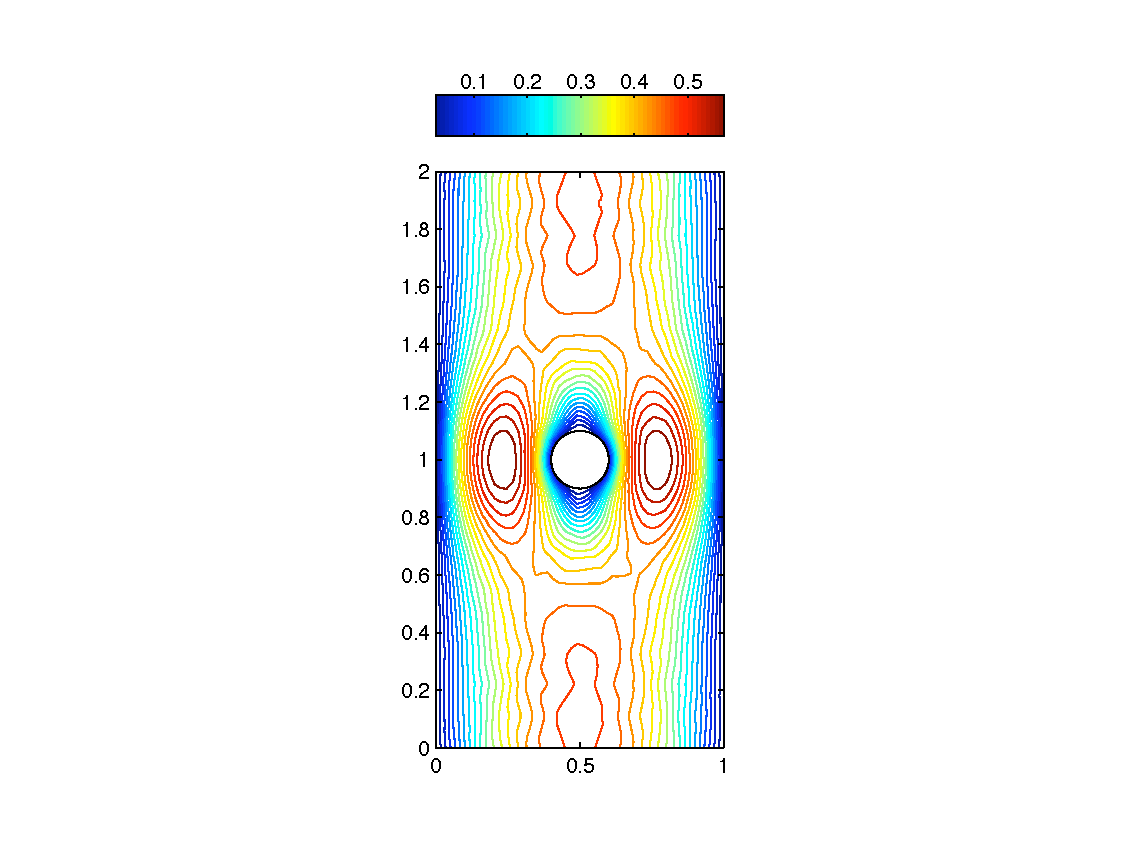
\includegraphics[width=10pc]{../plots/stokes_velocity_1.pdf}}
\subfigure[5 obstructions]{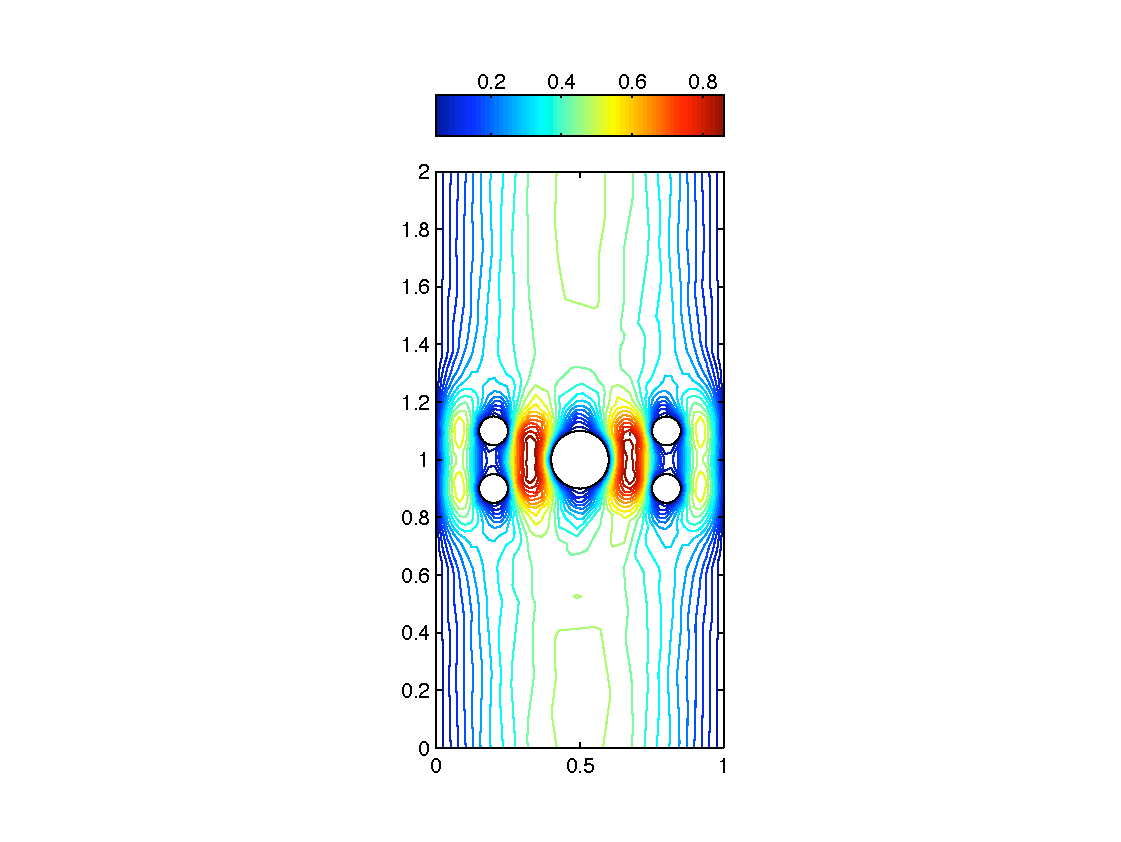
\includegraphics[width=10pc]{../plots/stokes_velocity_5.pdf}}
\subfigure[13 obstructions]{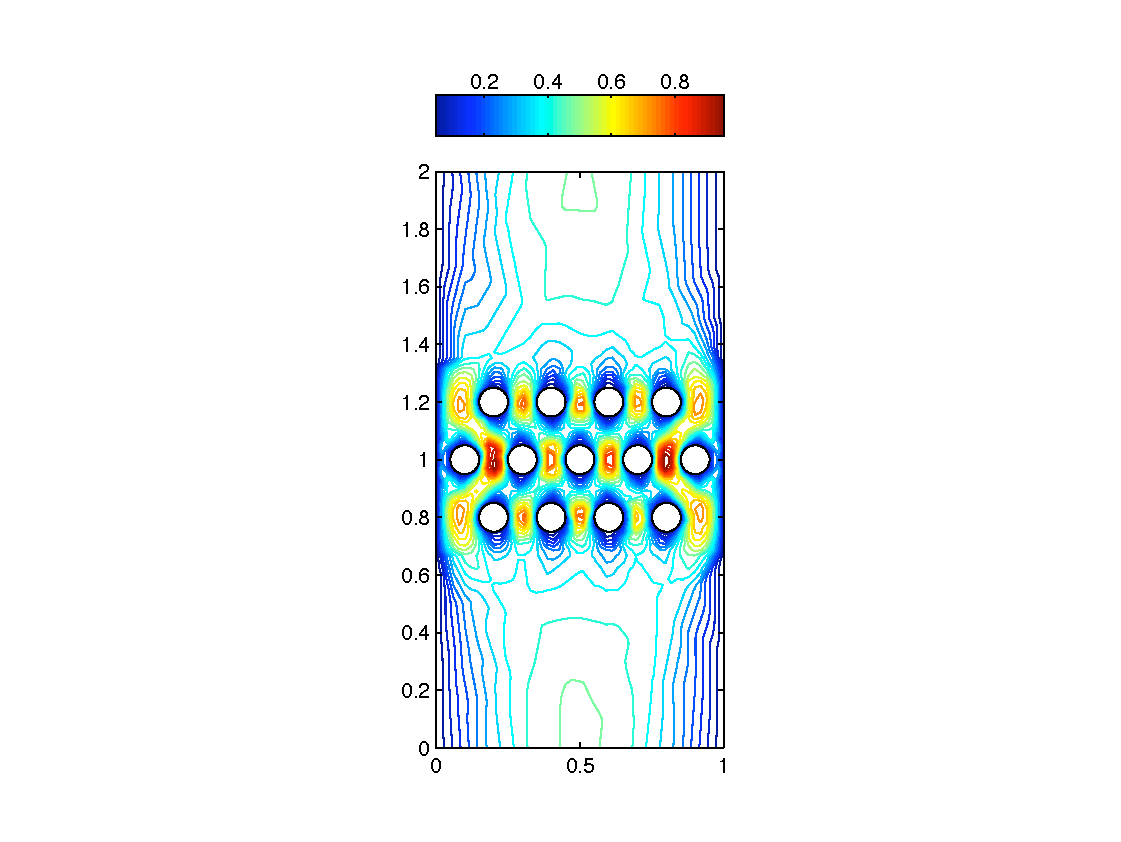
\includegraphics[width=10pc]{../plots/stokes_velocity_13.pdf}}
\caption{Velocity magnitude contours, $Re=1$}\label{fig:velocity}
\end{figure*}

\begin{figure*}
\centering
\subfigure[1 obstruction]{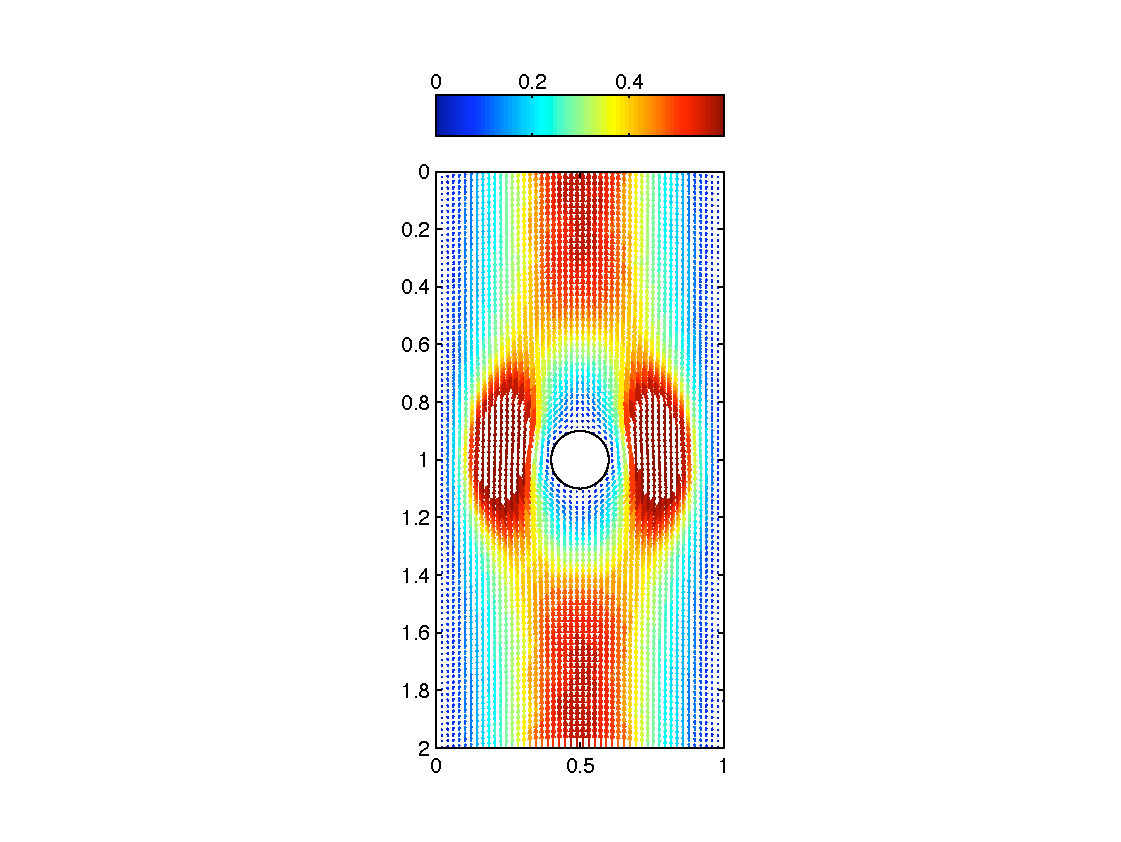
\includegraphics[width=10pc]{../plots/stokes_vectors_1.pdf}}
\subfigure[5 obstructions]{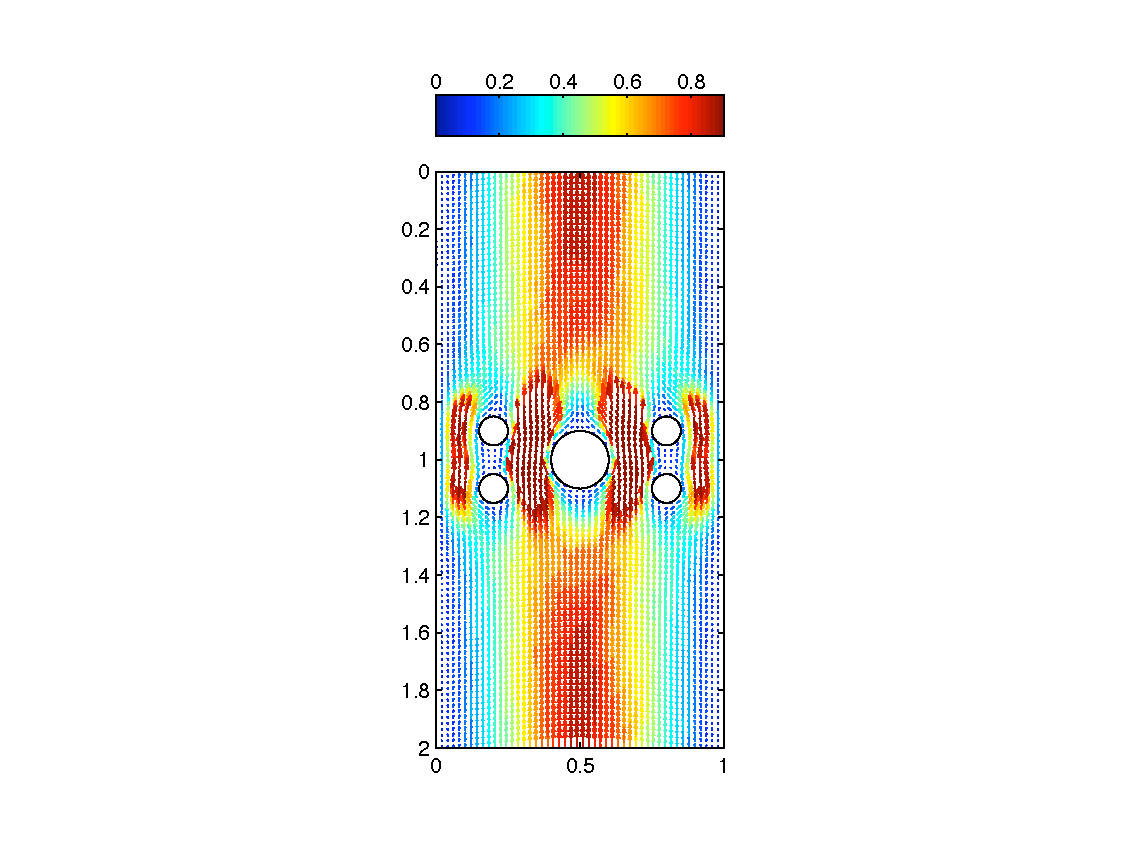
\includegraphics[width=10pc]{../plots/stokes_vectors_5.pdf}}
\subfigure[13 obstructions]{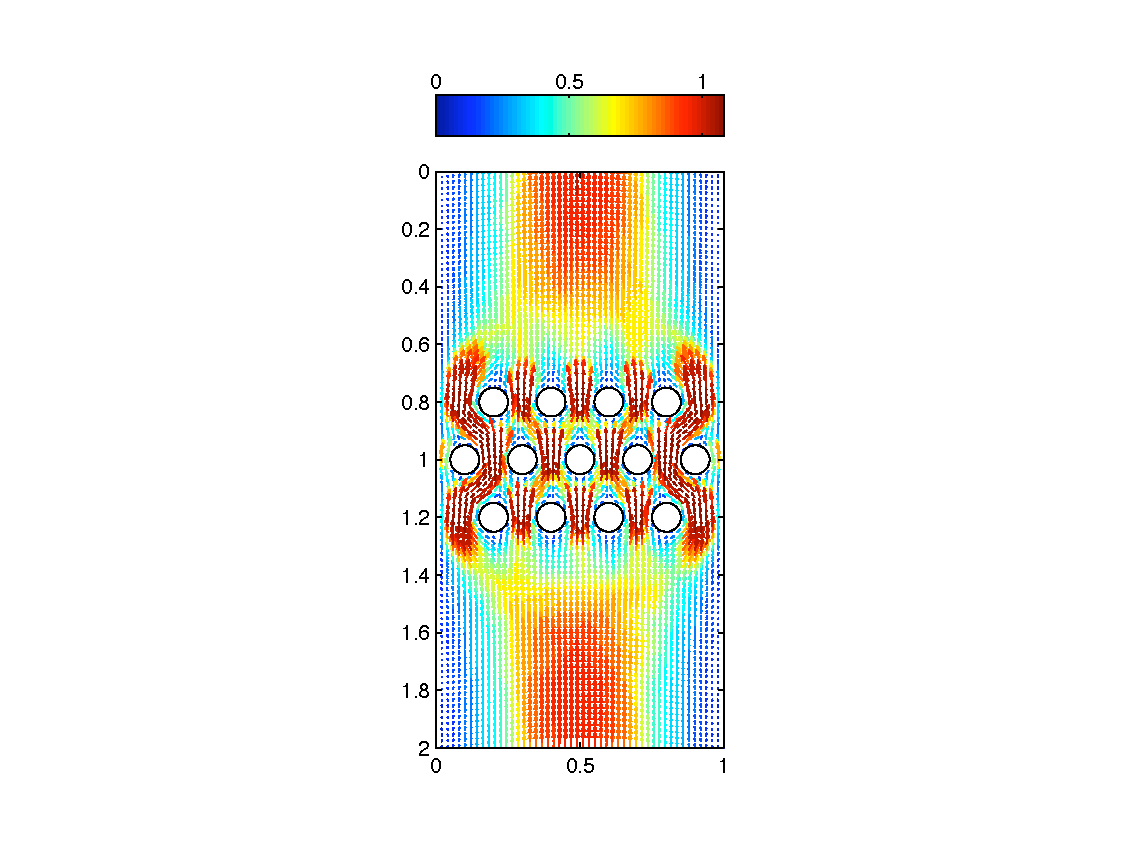
\includegraphics[width=10pc]{../plots/stokes_vectors_13.pdf}}
\caption{Velocity magnitude contours, $Re=1$}\label{fig:vectors}
\end{figure*}

\newpage
\begin{figure*}
\centering
%\noindent\subfigure[Velocity vectors with size proportional to their magnitude.]{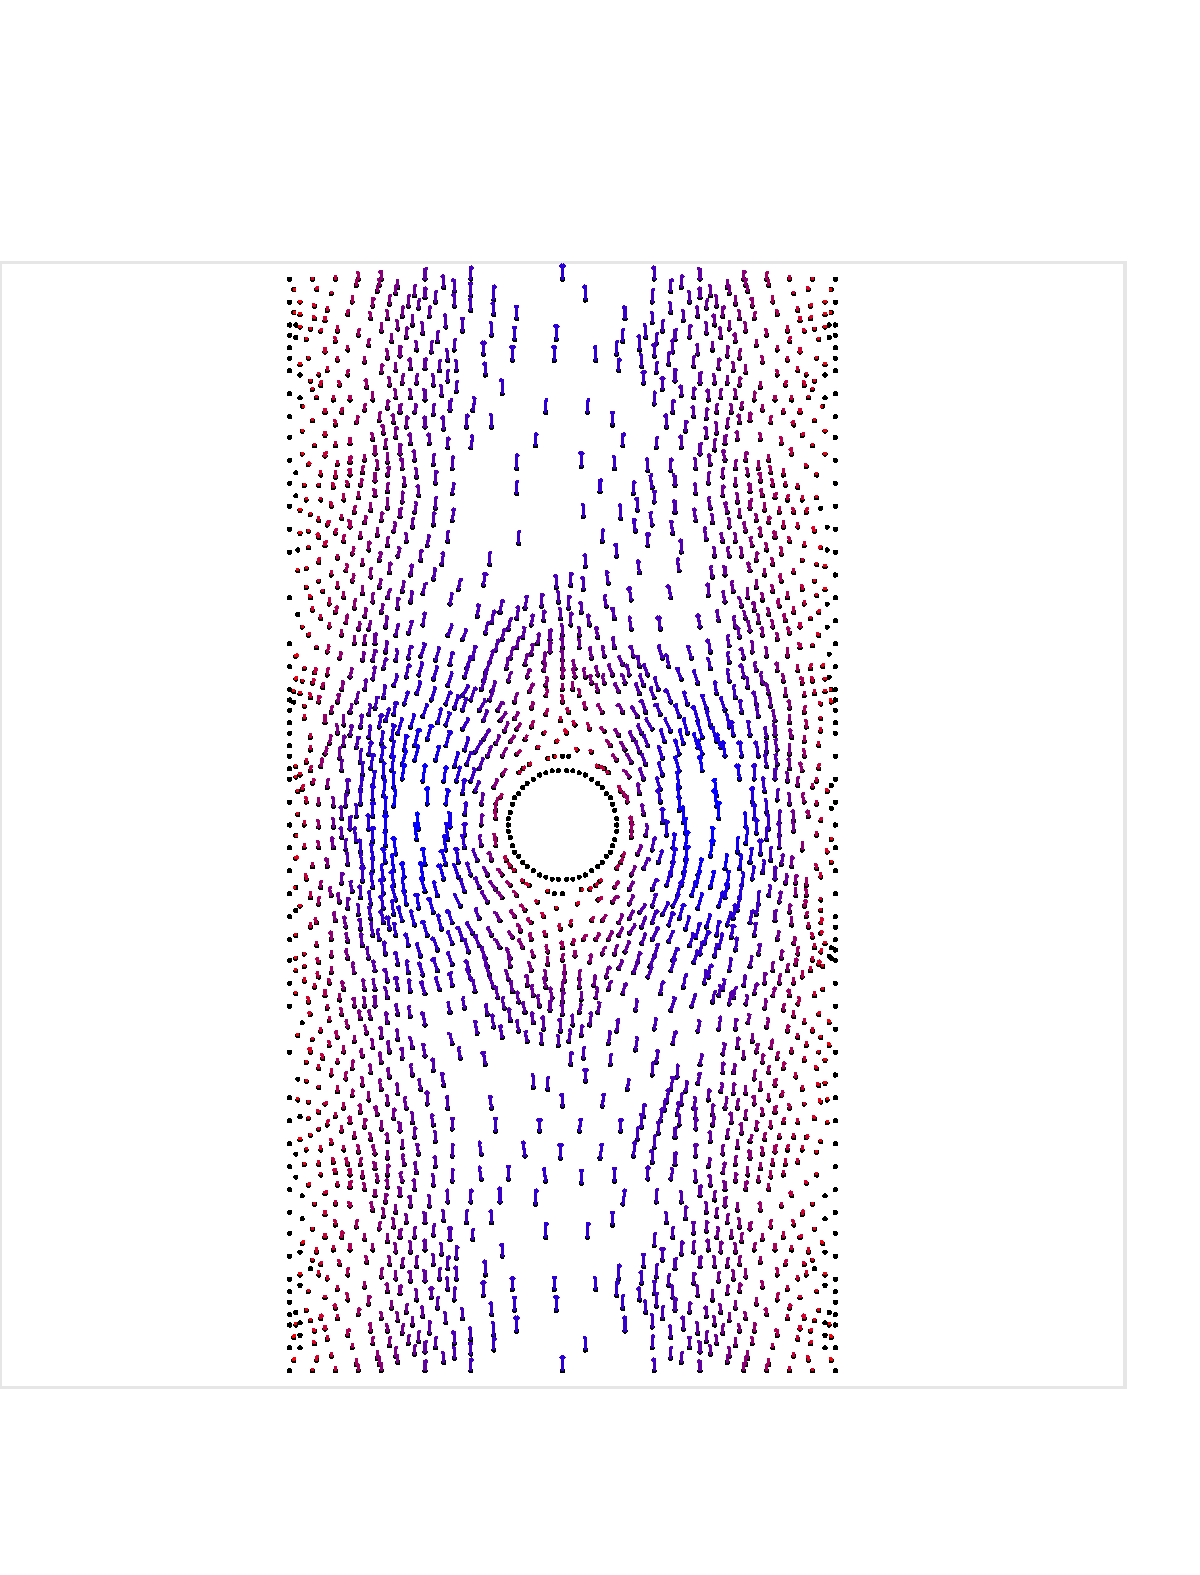
\includegraphics[width=13pc]{../plots/velocity_vec.pdf}}
\subfigure[0 obstructions]{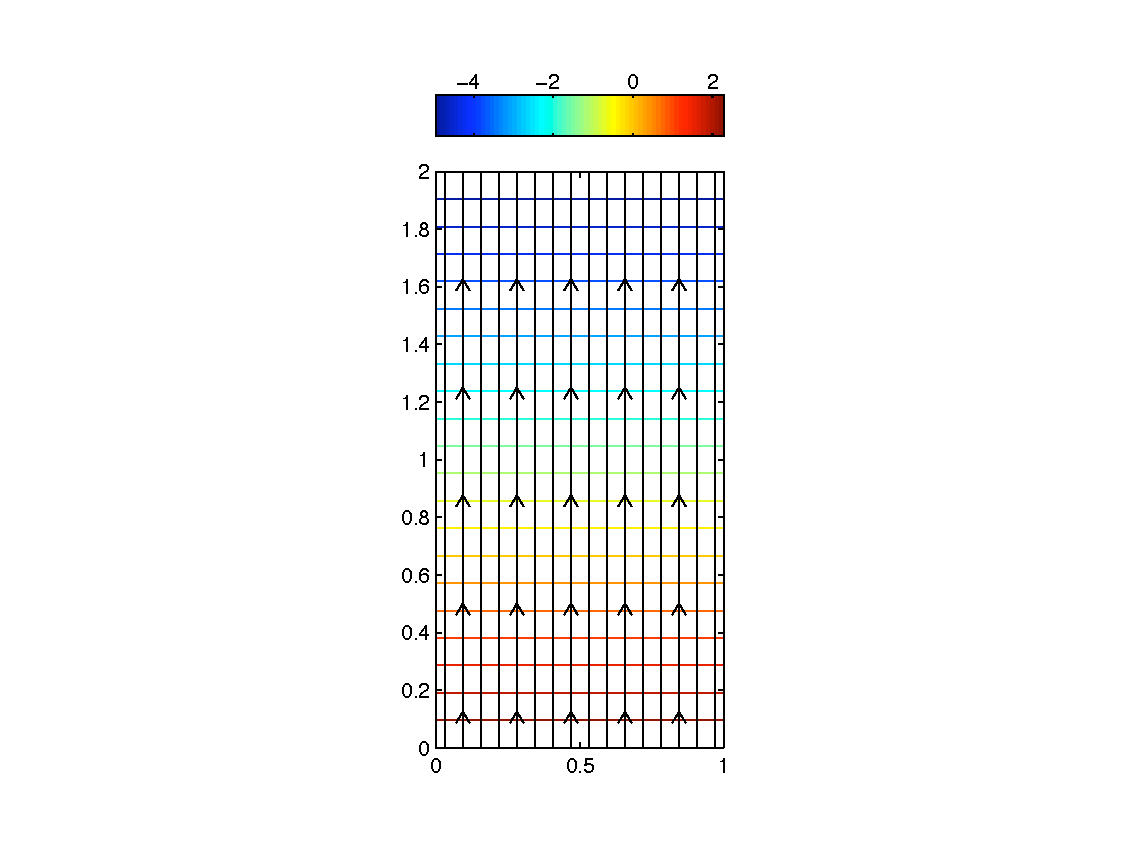
\includegraphics[width=10pc]{../plots/stokes_solution_0.pdf}}
\subfigure[1 obstruction]{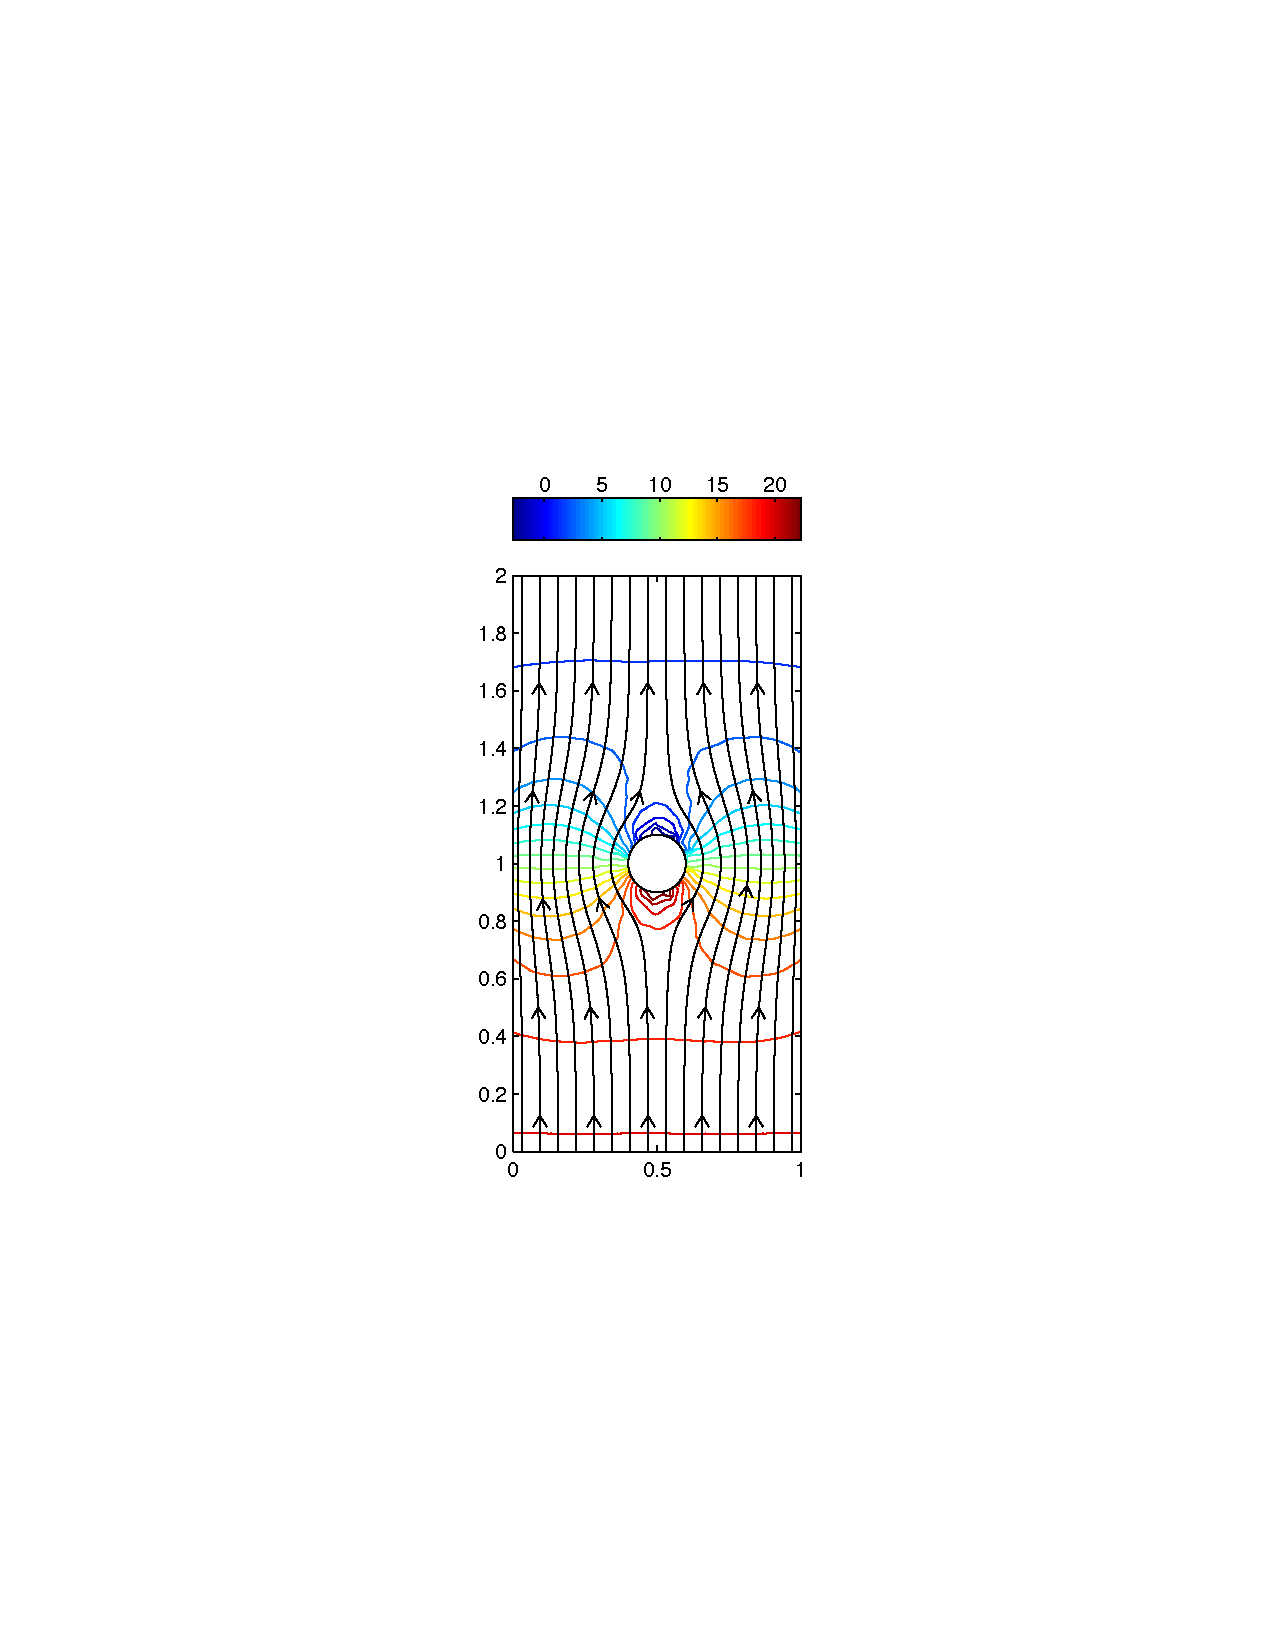
\includegraphics[width=10pc]{../plots/stokes_solution.pdf}}
\subfigure[5 obstructions]{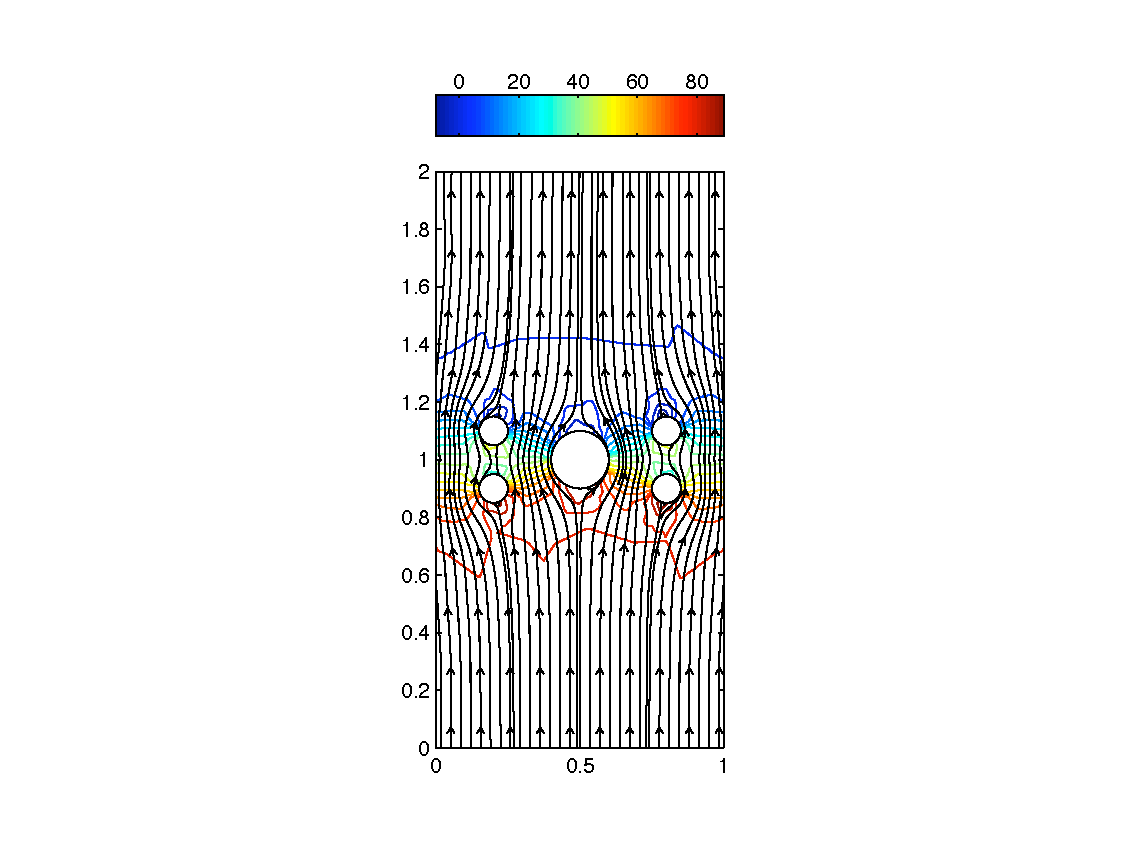
\includegraphics[width=9.9pc]{../plots/stokes_solution_5.pdf}}
\subfigure[13 obstructions]{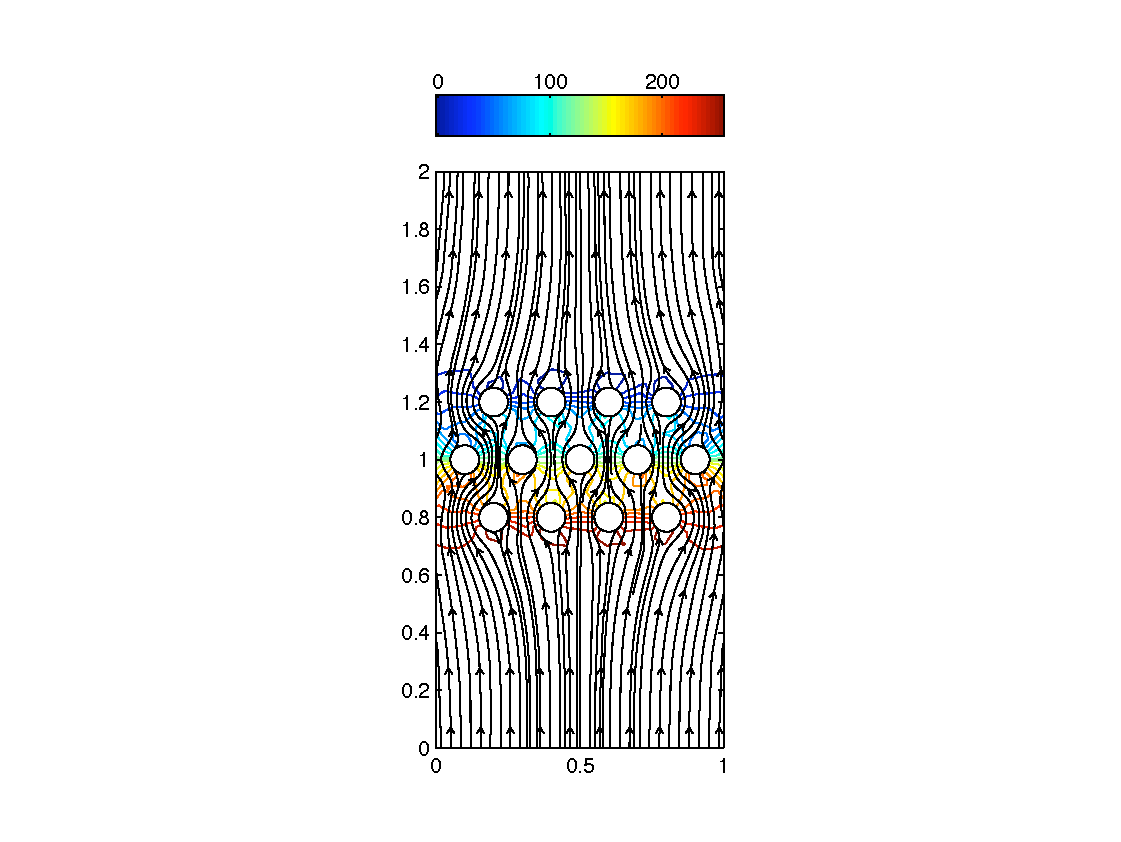
\includegraphics[width=10pc]{../plots/stokes_solution_13.pdf}}
\caption{Streamlines overlayed on pressure contours., $Re=1$}\label{fig:solution}
\end{figure*}

%\clearpage
\subsection{Adaptive Mesh Results}
Table \ref{tbl:1hole}, \ref{tbl:5holes}, \ref{tbl:13holes} show the details of the mesh refinement process with 1, 5 and 13 obstructions respectively.  With $\theta=p$ an optimal mesh was created in the fewest refinement steps with an average relative error on the final step of $\sim$18\% (Figure \ref{fig:err_1}).  With pressure as the error indicator, the mesh tended to be refined only locally around the cylinder (Figure \ref{fig:refine_p1}).  Using $\theta=v$ required 3 more refinement steps and over twice as many elements in the final mesh.  Using horizontal velocity as the error indicator tends to refine the mesh in a broad area around the cylinder (Figure \ref{fig:refine_u1}).  With $\theta=v$ the mesh tended to be refined near the left and right edges which are the no slip boundaries (Figure \ref{fig:refine_v1}).  

The plots of relative error (Figure \ref{fig:err_1},\ref{fig:err_5} and \ref{fig:err_13}) show that the average element was area limited ($A<A_{min}$) and not limited by the choice of $\epsilon$.  The imposition of a minimum area turned out to be crucial because in many elements the program ran out of precision before the acceptable error was achieved.  

For the arrangement of 5 cylinders using vertical velocity as the indicator generated the mesh containing the most elements but also he mesh with the lowest relative error (Figure \ref{fig:err_5}).  Once again using $\theta=u$ took the fewest refinement steps.  The generated meshes follow similar trends as with a single cylinder with the pressure indicator producing the most local refinement.  Fewer refinement steps were taken here because the mesh was more refined to begin with due to the nodes needed to define the cylinders.

For the array of 13 cylinders, the mesh was well defined to begin with and so the refinement process using pressure and horizontal velocity was not able to make much improvement on the average relative error.  Despite this, pressure still achieved the lowest average relative error in the fewest refinement steps.  \vfill

\begin{table*}
\flushleft
\caption{One obstruction, refinement details}\label{tbl:1hole}
\begin{tabular}{cccccccccc}
\toprule
&& $\theta=u$& &&$\theta=v$& & &$\theta=p$&\\   
Refinement Step & Elements & Nodes & Unknowns & Elements & Nodes & Unknowns & Elements & Nodes & Unknowns\\
\midrule
1 & 88 & 214   & 491  & 88   & 214  & 491  & 88  & 214  & 491 \\
2 & 161 & 361  & 822  & 180  & 406  & 925  & 178 & 402  & 916\\
3 & 300 & 642  & 1455 & 346  & 752  & 1707 & 332 & 722  & 1639 \\
4 & 482 & 1008 & 2279 & 687  & 1467 & 3324 & 465 & 1003 & 2275 \\
5 & 597 & 1241 & 2804 & 939  & 1971 & 4458 & --  & --   & -- \\
6 & 619 & 1285 & 2903 & 1013 & 2119 & 4791 & --  & --   & -- \\
7 & --  & --   & --   & 1027 & 2147 & 4854 & --  & --   & -- \\
\bottomrule
\end{tabular}
\end{table*}

\begin{table*}
\flushleft
\caption{Five obstructions, refinement details}\label{tbl:5holes}
\begin{tabular}{cccccccccc}
\toprule
&& $\theta=u$& &&$\theta=v$& & &$\theta=p$&\\   
Refinement Step & Elements & Nodes & Unknowns & Elements & Nodes & Unknowns & Elements & Nodes & Unknowns\\
\midrule
1 & 189 & 455 & 1041 & 189 & 455 & 1041 & 189 & 455 & 1041 \\
2 & 301 & 683 & 1555 & 318 & 718 & 1634 & 285 & 651 & 1483 \\
3 & 405 & 897 & 2038 & 440 & 978 & 2233 & 309 & 705 & 1606 \\
4 & 440 & 970 & 2203 & 598 & 1308 & 2969 & 315 & 717 & 1633 \\
5 & 450 & 990 & 2248 & 674 & 1464 & 3321 & -- & -- & --\\
\bottomrule
\end{tabular}
\end{table*}

\begin{table*}
\flushleft
\caption{Thirteen obstructions, refinement details}\label{tbl:13holes}
\begin{tabular}{cccccccccc}
\toprule
&& $\theta=u$& &&$\theta=v$& & &$\theta=p$&\\   
Refinement Step & Elements & Nodes & Unknowns & Elements & Nodes & Unknowns & Elements & Nodes & Unknowns\\
\midrule
1 & 299 & 735 & 1682 & 299 & 735 & 1682 & 299 & 735 & 1682 \\
2 & 438 & 1016 & 2315 & 506 & 1162 & 2646 & 380 & 900 & 2054 \\
3 & 488 & 1120 & 2550 & 616 & 1392 & 3166 & 392 & 924 & 2108 \\
4 & 516 & 1176 & 2676 & 712 & 1596 & 3628 & 398 & 936 & 2135 \\
5 & -- & -- & -- & 741 & 1659 & 3771 & -- & -- &  \\
\bottomrule
\end{tabular}
\end{table*}





\begin{figure}
\noindent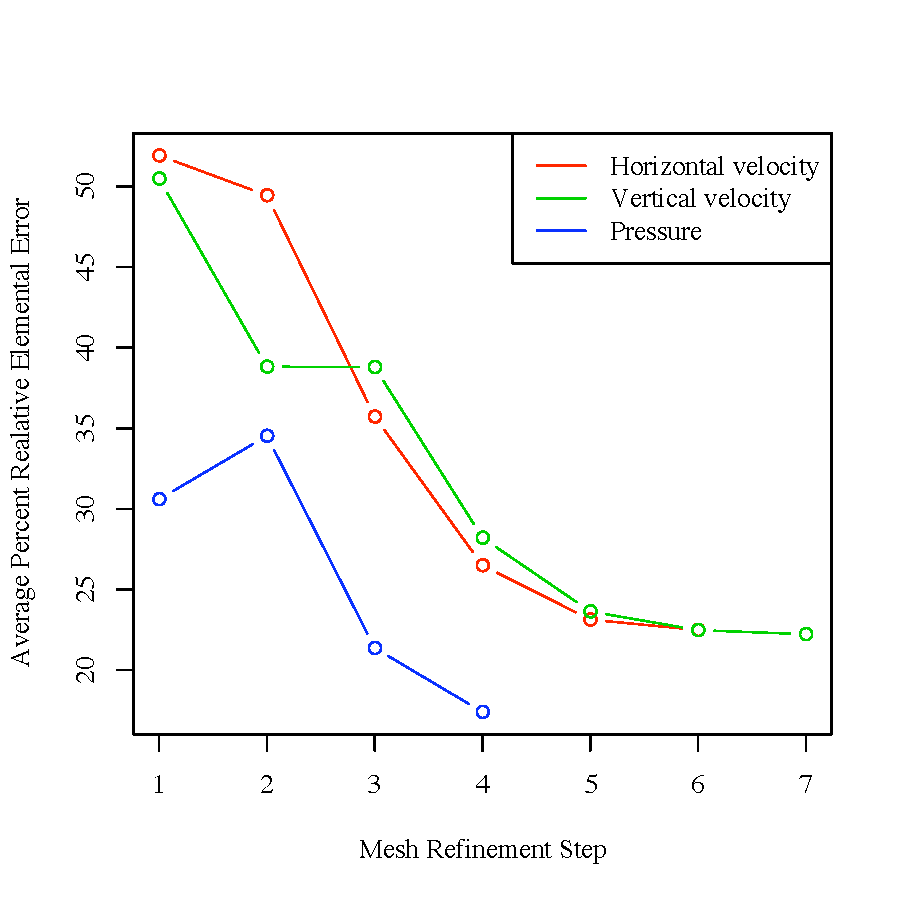
\includegraphics[width=20pc]{../plots/errorstep_1.pdf}
\caption{Average relative element error as a function of refinement step for 1 obstructions.}\label{fig:err_1}
\end{figure}

\begin{figure}
\noindent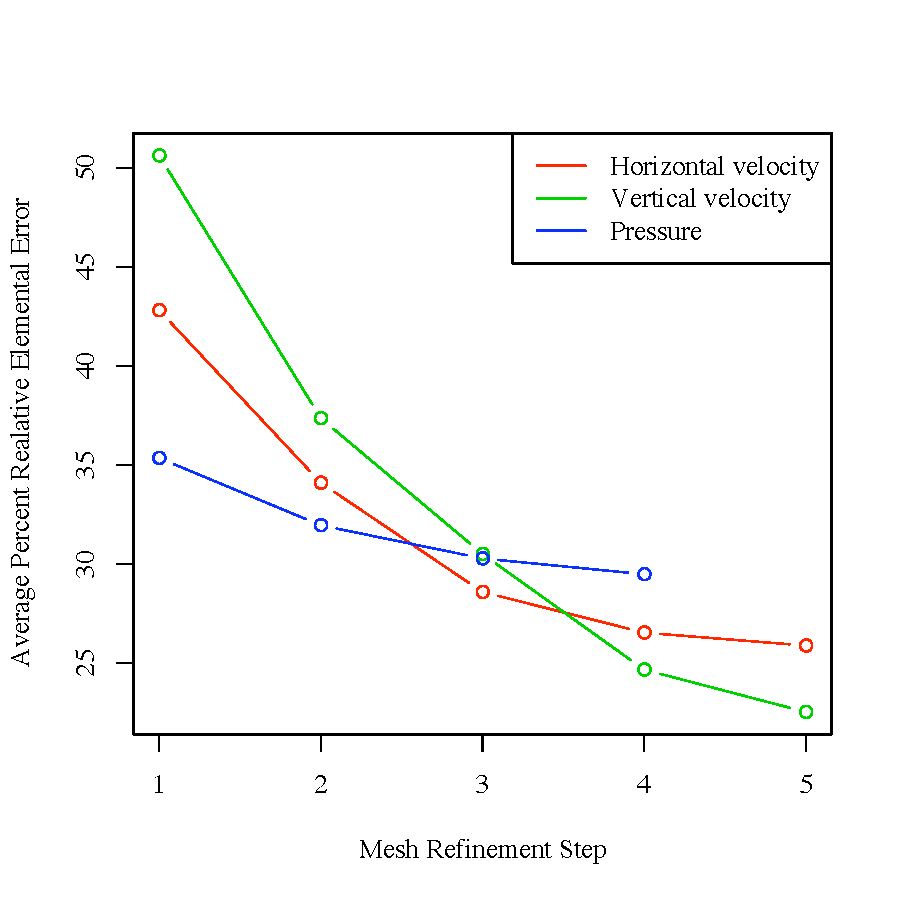
\includegraphics[width=20pc]{../plots/errorstep_5.pdf}
\caption{Average relative element error as a function of refinement step for 5 obstructions.}\label{fig:err_5}
\end{figure}

\begin{figure}
\noindent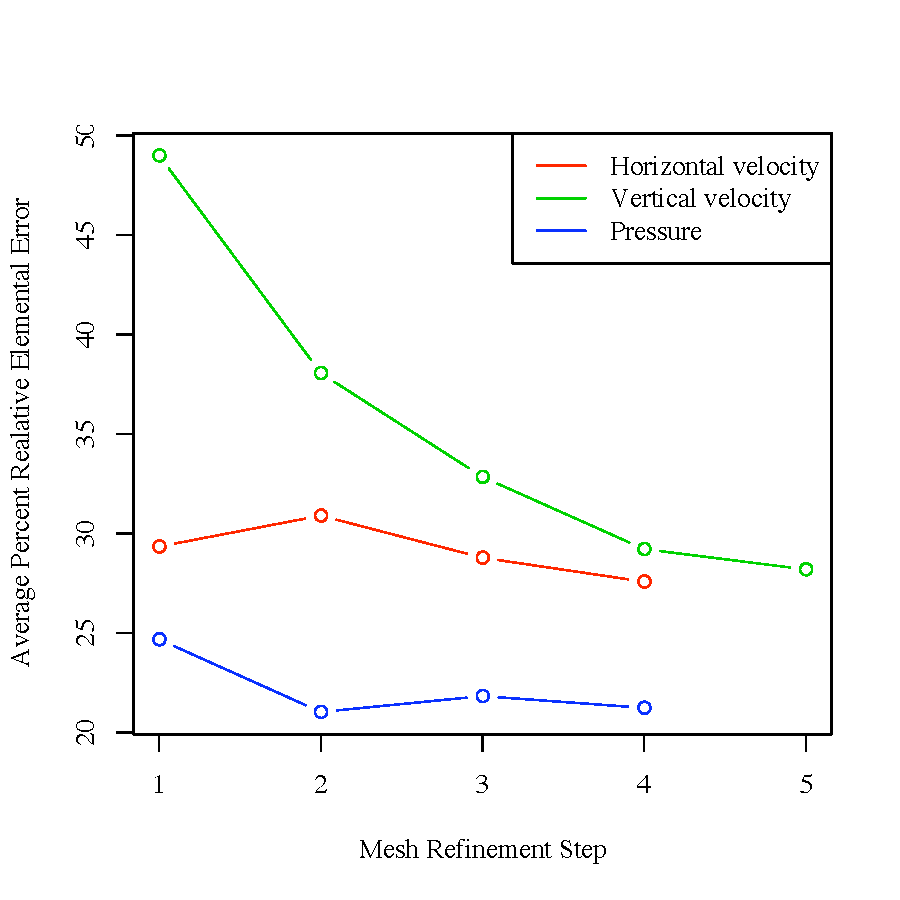
\includegraphics[width=20pc]{../plots/errorstep_13.pdf}
\caption{Average relative element error as a function of refinement step for 13 obstructions.}\label{fig:err_13}
\end{figure}


%\begin{figure}
%\noindent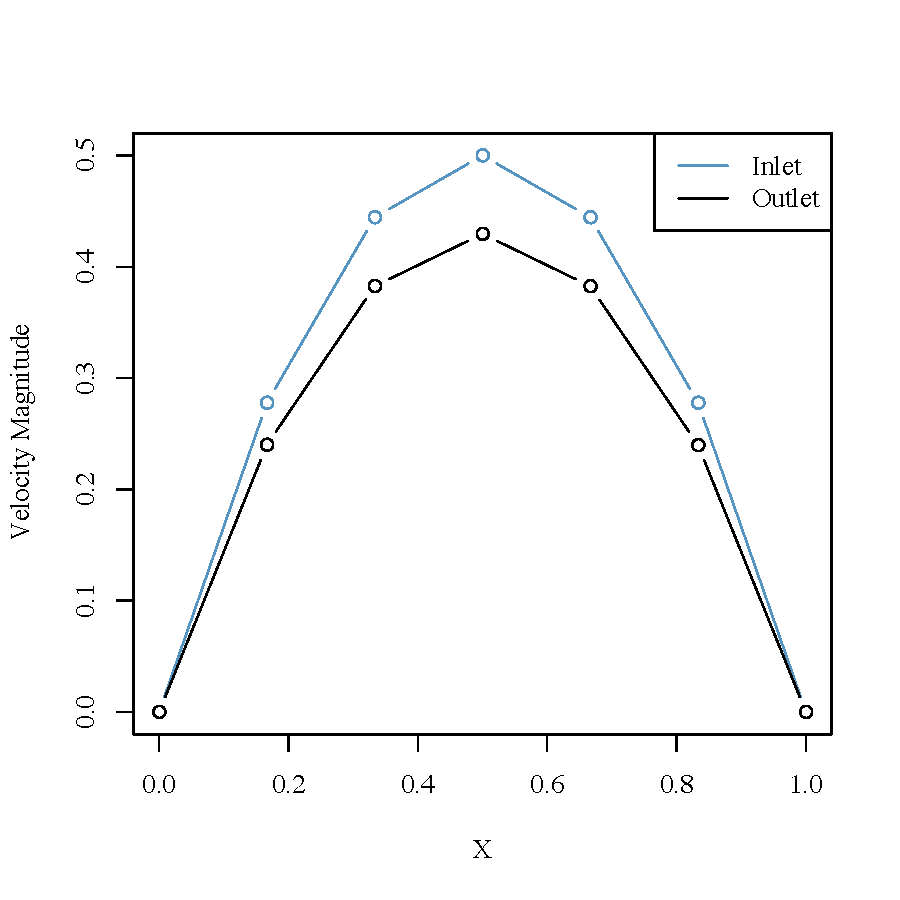
\includegraphics[width=20pc]{../plots/vel_profile_1.pdf}
%\caption{Velocity profile at the inlet and outlet of with one obstruction}
%\end{figure}

\subsection{Sparseness and Computation Time}
The assumption that the coefficient matrix resulting from an unstructured adaptive mesh refinement process would be sparse and unbanded turned out to be a good one.  Figure \ref{fig:sparseity} is a visualization of a sample coefficient matrix with points in the nonzero entries.  The coefficient matrix contained $>99.99$\% zero entries, that is $<.001$\% of the entries were zero.  This was typical for the Stokes stiffness matrices. 

\begin{figure}
\noindent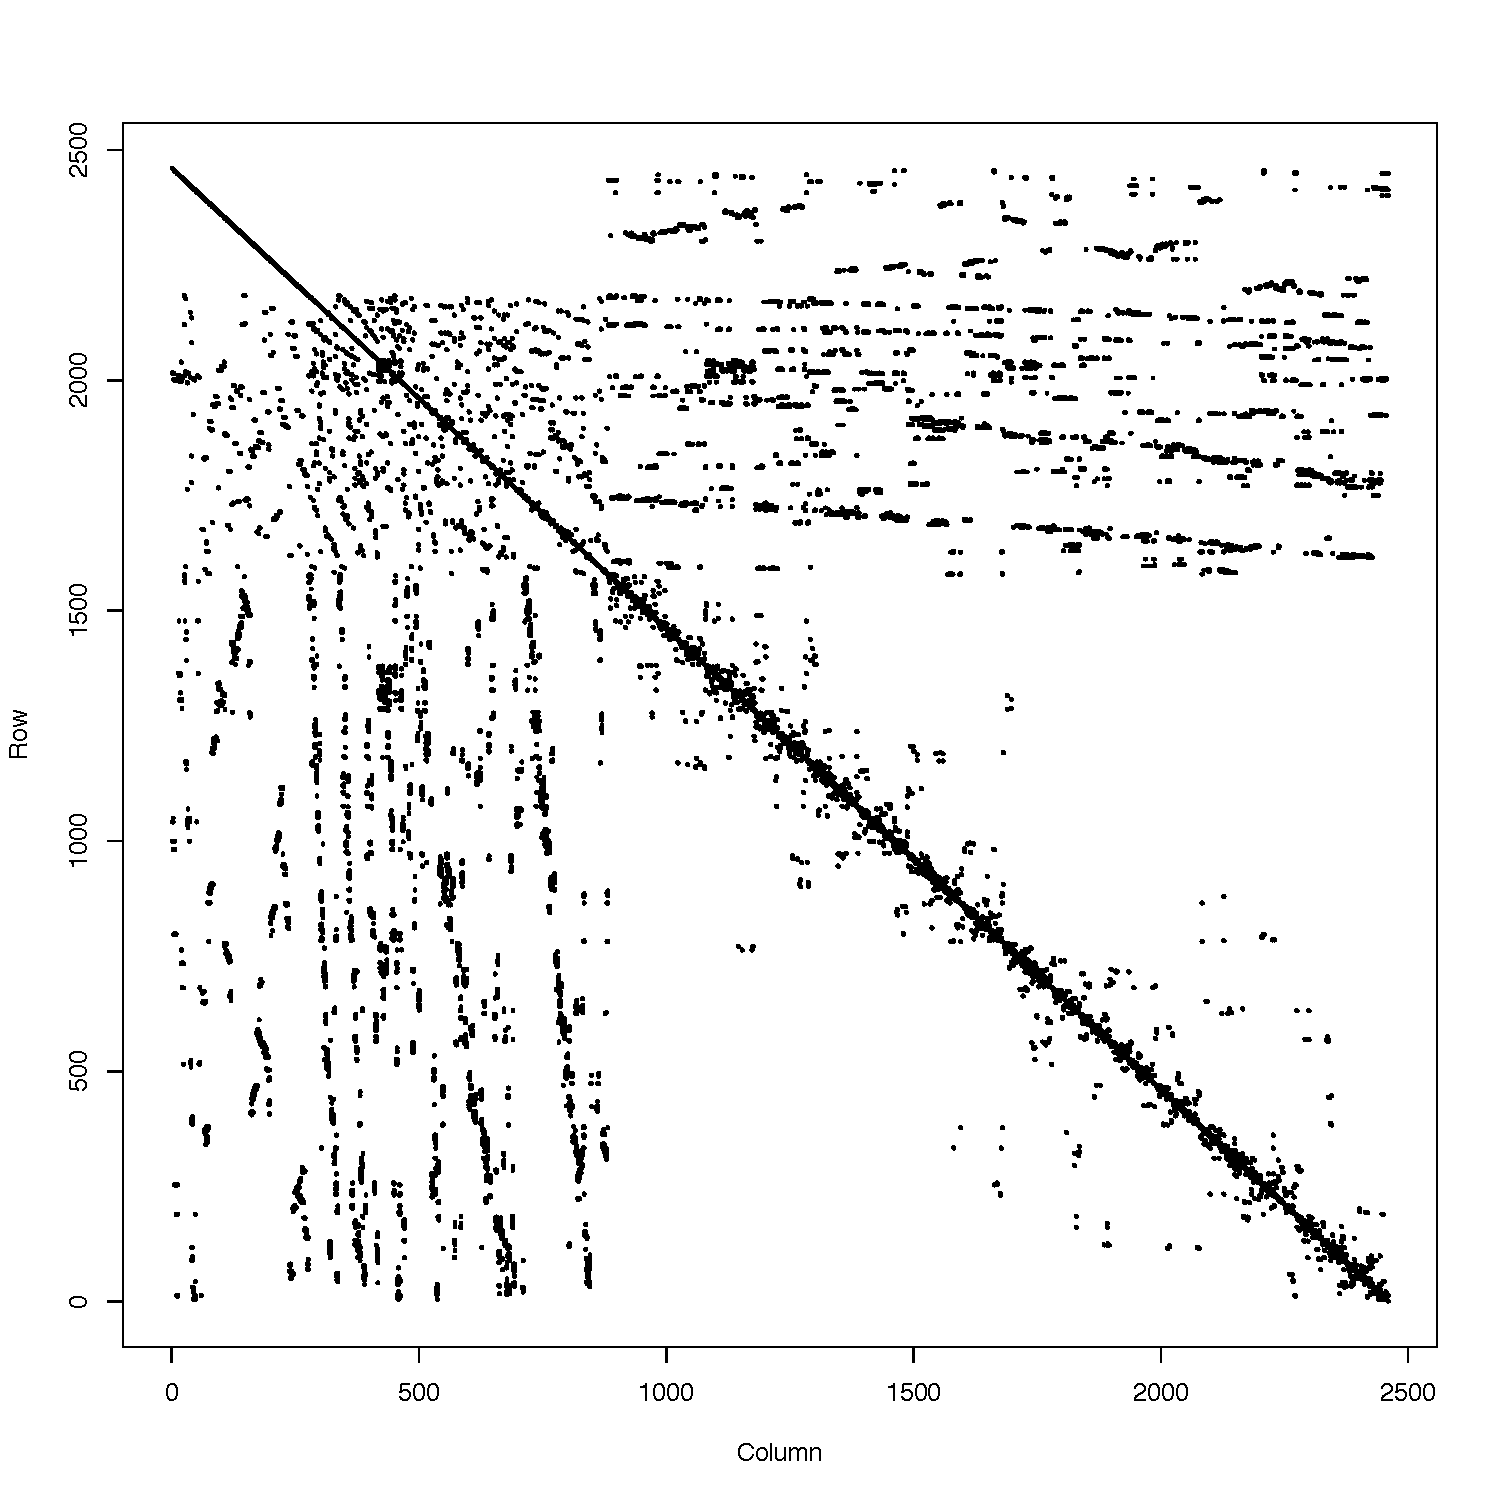
\includegraphics[width=20pc]{../plots/sparse_small.pdf}[h]
\caption{Sample coefficient matrix with points in the nonzero entries}\label{fig:sparseity}
\end{figure}

The assertion earlier in the paper was that dense matrix storage and therefore solution time increases as $N^2$ where sparse storage increases linearly with $N$.  We see from the solution times that tis is indeed the case (Figure \ref{fig:times}).  Times are from 64-bit Intel Core II Duo processor.  Figure \ref{fig:times} does not clearly show it but the {\tt  LAPACK} dense matrix solver is actually faster when the $N \lesssim 1000$.  In this case though solution times for both sparse and dense solvers were less than 1 second.

\begin{figure}
\noindent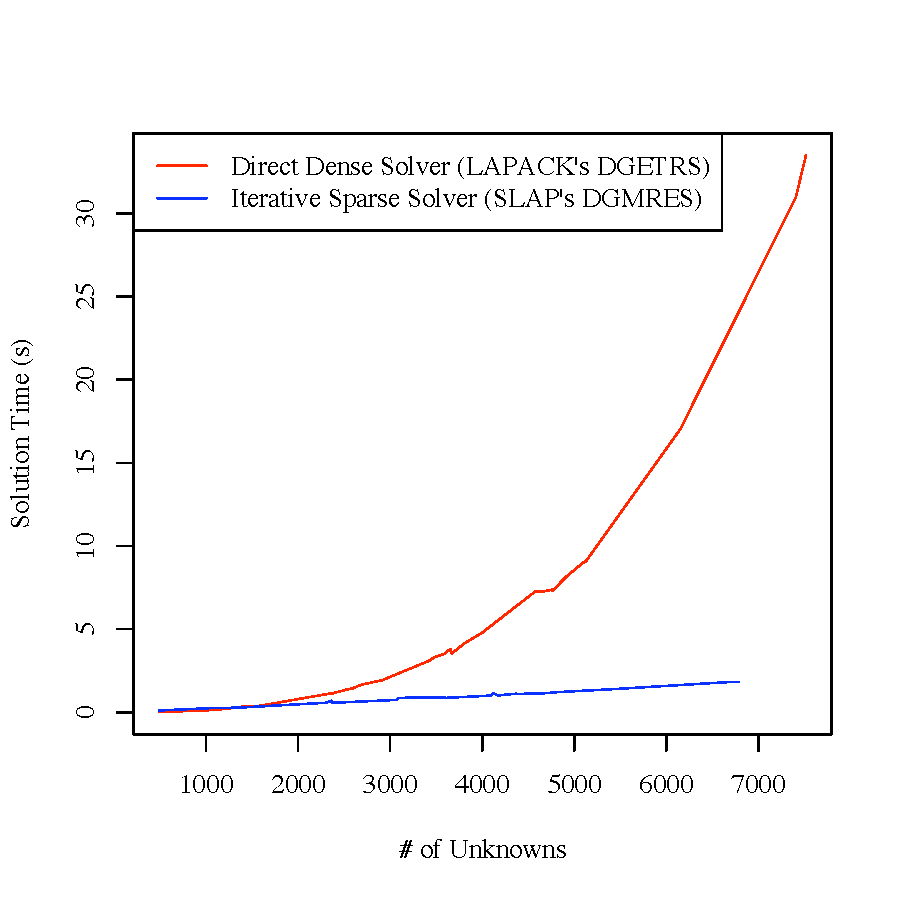
\includegraphics[width=20pc]{../plots/solution_times.pdf}
\caption{Solution times of direct versus sparse method}\label{fig:times}
\end{figure}




\section{Conclusions}

Pressure is a good error indicator.  Sparse storage crucial.  YO MAMMA.

%%% End of body of article:

%%%%%%%%%%%%%%%%%%%%%%%%%%%%%%%%
%% Optional Appendix goes here
%
%%%%%%%%%%%%%%%%%
% Geophysical Research Letters only allows an appendix without a letter.
%% You can get this result with 
%  \section*{Appendix} 
%  or 
%  \section*{Appendix: Title}
%%%%%%%%%%%%%%%%%
%
% \appendix resets counters and redefines section heads
% but doesn't print anything. 
% After typing  \appendix 
%
% \section{Here Is Appendix Title}
% will print 
% Appendix A: Here Is Appendix Title
%
% \section*{Appendix}
% will print 
% Appendix 
%
% \section*{Appendix: Here Is Appendix Title}
% will print 
% Appendix: Here Is Appendix Title 
%
% For only 1 appendix \appendix \section{Appendix} is preferred.
% which will print 
% Appendix A

%%%%%%%%%%%%%%%%%%%%%%%%%%%%%%%%%%%%%%%%%%%%%%%%%%%%%%%%%%%%%%%%
%
% Optional Glossary or Notation section, goes here
%
%%%%%%%%%%%%%%
% Glossary only allowed in Reviews of Geophysics
% \section*{Glossary}
% \paragraph{Term}
% Term Definition here
%
%%%%%%%%%%%%%%
% Notation -- End each entry with a period.
 \begin{notation}
 $\rho$ & Fluid Density.\\
 $\rho_t$ & Time derivative of density.\\
 ${\bf V}$ & Velocity vector.\\
 ${\bf V}_t$ & Time derivative of velocity vector.\\
 $\nabla$ & Partial derivative operator.\\
 $\nabla^2$ & Second derivative operator.\\
 $p$ & Fluid pressure.\\
 $\mu$ & Dynamic Viscocity.\\
 $\nu$ & kinematic Viscocity.\\
 $\mathcal{E}_e$ & Actual error over element $e$.\\
 $E_e$ & Error estimate over element $e$.\\
 $A$ & Finite element coefficient matrix or alternately the area of a given finite element.\\
 $n_s$ & Number of nonzero entries in A.\\
 $N$ & Order of A.\\
 $E_e$ & Error estimate over element $e$.\\
 $Re$ & Reynolds number.\\
 $\hat{\mathbf{V}}$ & Piecewise continuous approximation of $\mathbf{V}$.\\
 $\tilde{\mathbf{V}}$ & Nodal value of velocity vector.\\
 $\phi_i$ & Velocity interpolating function.\\
 $\hat{p}$ & Piecewise continuous approximation of $p$.\\
 $\tilde{p}$ & Nodal value of pressure.\\
 $\psi_i$ & Pressure interpolating function.\\
 $n_v$ & number of velocity nodes.\\
 $n_p$ & number of pressure nodes.\\
 $\mathbf{w}_i$ & FE weighting functions.\\
 $\mathcal{L}$ & Stokes operator.\\
 $\Omega$ & Problem domain.\\
 $\p\Omega$ & Boundary of problem domain.\\
 $B$ & General function defined on $\Omega$.\\
 $\mathbf{F}$ & General vector field defined on $\Omega$.\\
 $\mathbf{n}$ & Outward pointing unit normal vector on $\p\Omega$.\\
 $\mathbf{g}$ & Right hand side vector.\\
 $\mathbf{g}$ & Vector of unknown nodal values.\\
 $\mathbf{\tilde{u}}$ & Vector of unknown nodal values of horizontal velocity.\\
 $\mathbf{\tilde{v}}$ & Vector of unknown nodal values of vertical velocity.\\
 $\mathbf{\tilde{p}}$ & Vector of unknown nodal values of pressure.\\
 $\theta_n$ & Error indicator at node $n$.\\
 $h_e$ & length scale of element $e$.\\
 $A_{min}$ & Minimum allowable element area.\\
 $\epsilon$ & Maximum allowable percent relative error.\\
 $m$ & Maximum allowable number of elements which do not meet the error or area criteria.\\
 $L_x$ & Length of domain in $x$ direction.\\
 $L_y$ & Length of domain in $y$ direction.\\
 $u$ & Horizontal component of velocity.\\
 $v$ & Vertical component of velocity.\\
 $k$ & Inlet velocity scaling coefficient.\\
 $(x_o,y_o)$ & Point at which pressure is specified.\\
 $T_r$ & Reference triangle in dimensionless coordinates.\\
 $T$ & Actual triangle in global cartesian coordinates.\\
 $(\xi,\eta)$ & Dimensionless (natural coordinates).\\
 $(\xi_p,\eta_p)$ & Qquadriture point in dimensionless coordinates.\\
 $w_p$ & Gaussian quadriture weights.\\
 $A_T$ & Area of triangle $T$.\\
 \end{notation}
%%%%%%%%%%%%%%%%%%%%%%%%%%%%%%%%%%%%%%%%%%%%%%%%%%%%%%%%%%%%%%%%
%
%  ACKNOWLEDGMENTS
%%%%%%%%%%%%%%%%%%%%%%%%%%%%%%%%%%%%%%%%%%%%%%%%%%%%%%%%%%%%%%%%%
\begin{acknowledgments}
This template was typeset in pdf\LaTeX{} and was modified from the  AGU template available at \\{\tt http://www.agu.org/pubs/helpdesk/index.html}
\end{acknowledgments}

%%%%%%%%%%%%%%%%%%%%%%%%%%
\bibliography{refs}
\vfill
%%%%%%%%%%%%%%%%%%%%%

\newpage
\appendix 
\section{Refinement plots}
 \newcommand{\w}{6.1pc}
 \newcommand{\h}{12pc}
%%%%%%%%%%%%%%%%% 
%
%		1 holes
%
%%%%%%%%%%%%%%%%%
\begin{figure}[h]
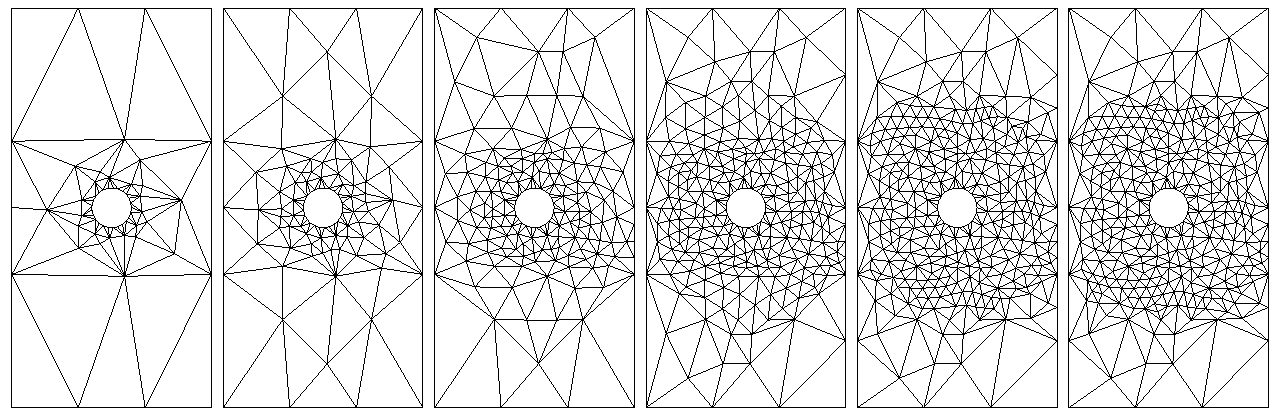
\includegraphics[height=\h]{../plots/u_1_row.pdf}
%\noindent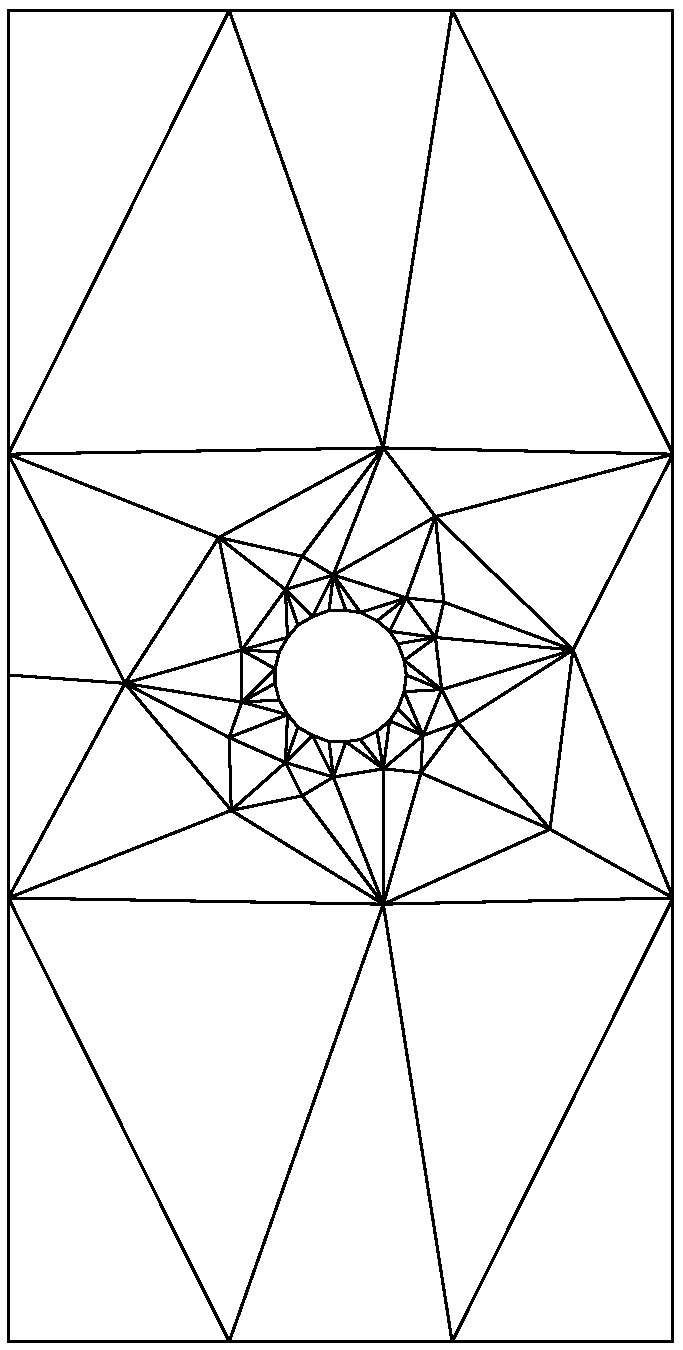
\includegraphics[width=\w]{../plots/mesh1ele_u.pdf}
%\noindent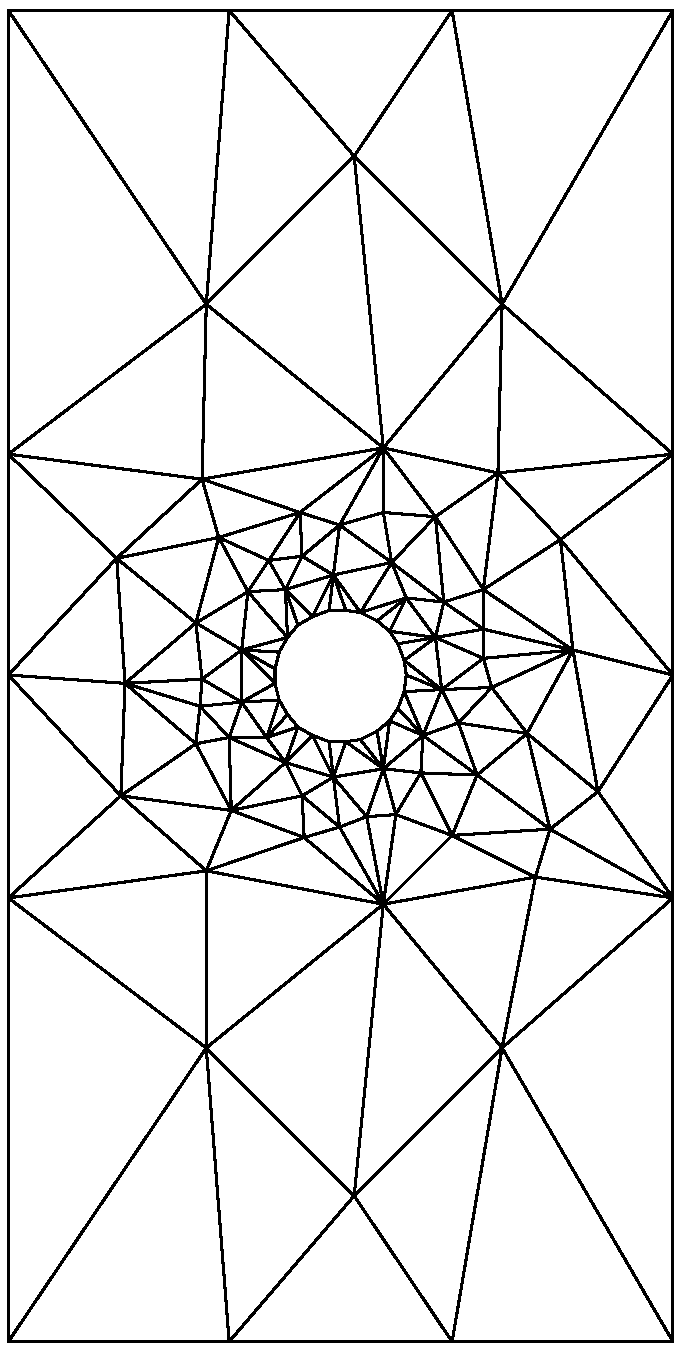
\includegraphics[width=\w]{../plots/mesh2ele_u.pdf}
%\noindent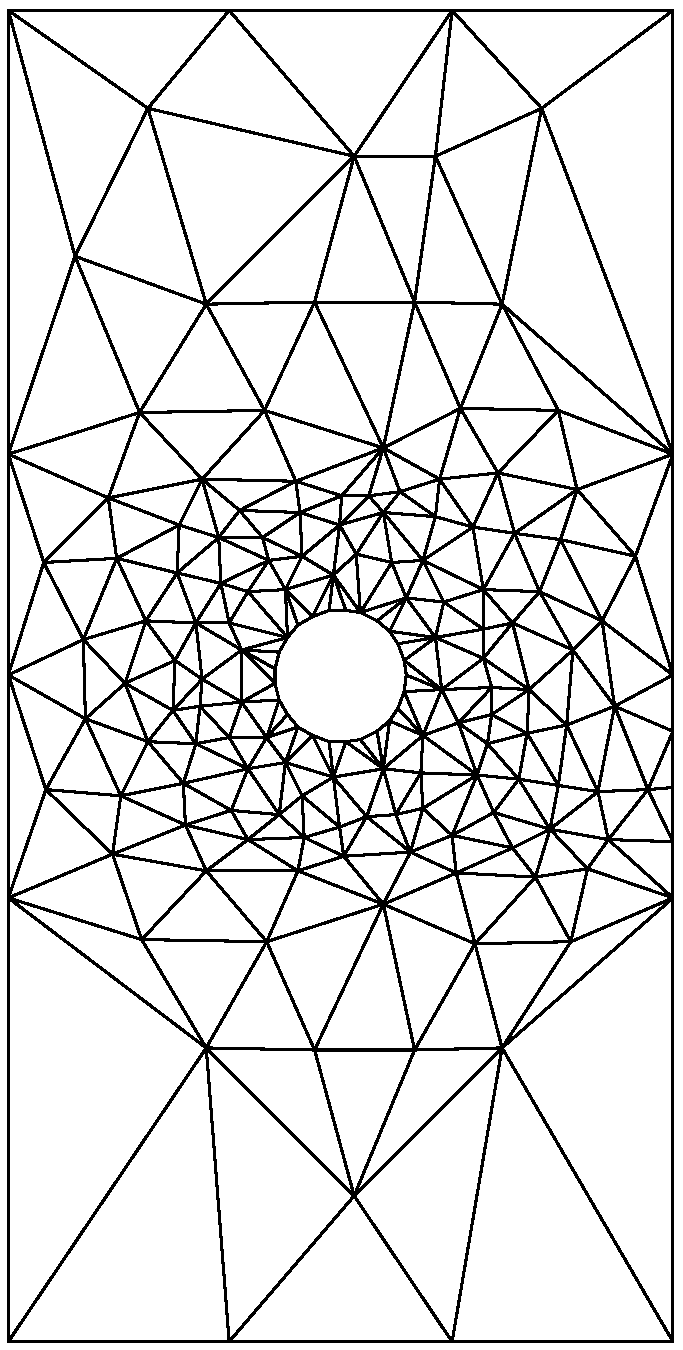
\includegraphics[width=\w]{../plots/mesh3ele_u.pdf}
%\noindent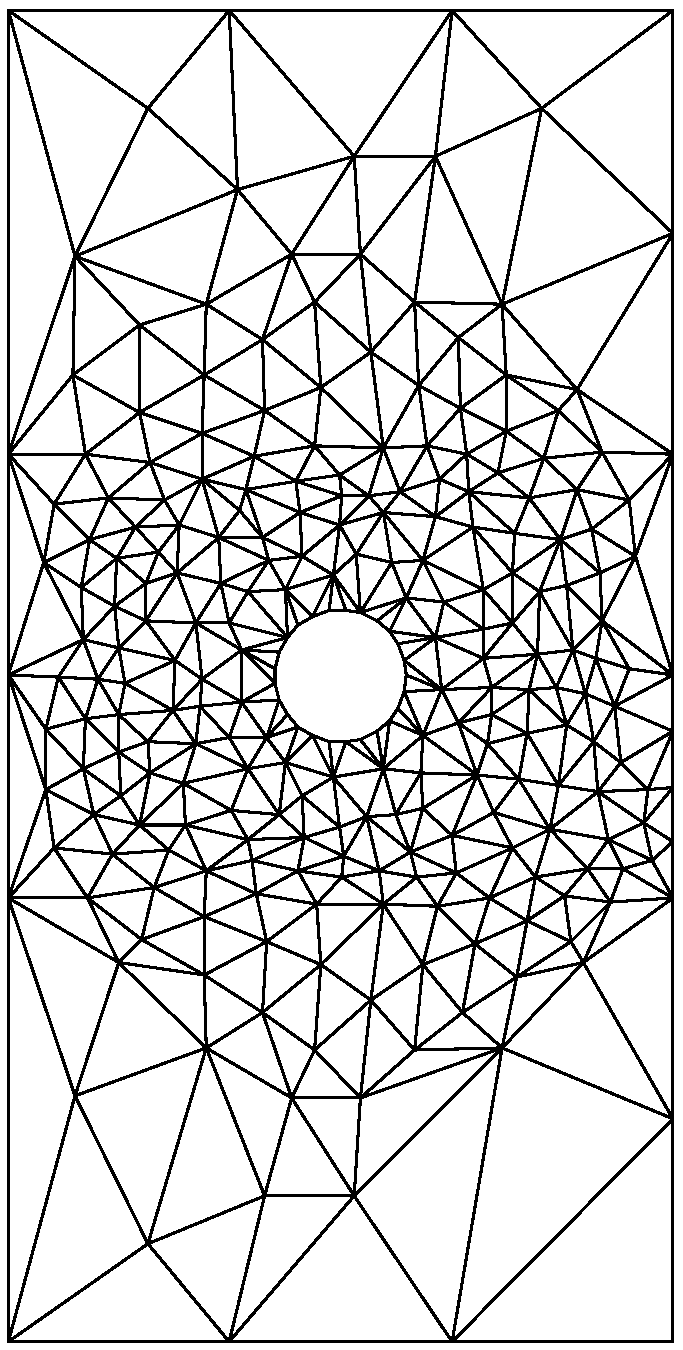
\includegraphics[width=\w]{../plots/mesh4ele_u.pdf}
%\noindent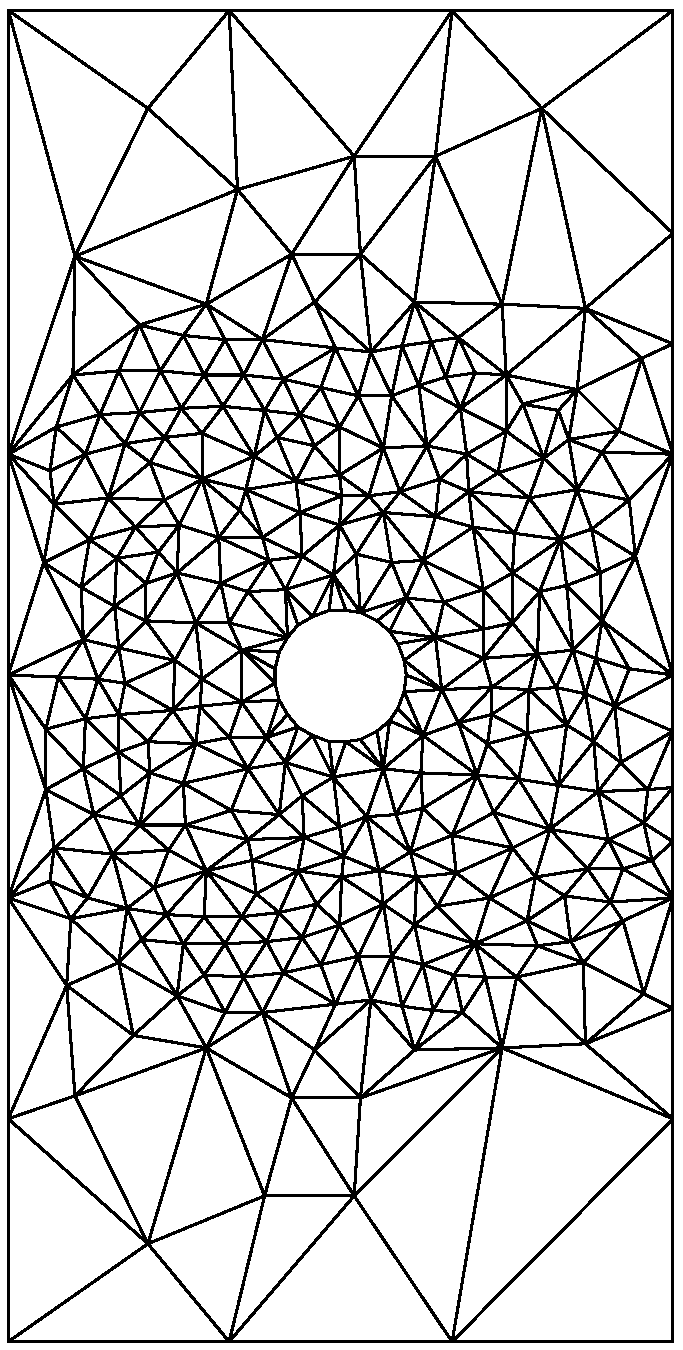
\includegraphics[width=\w]{../plots/mesh5ele_u.pdf}
%\noindent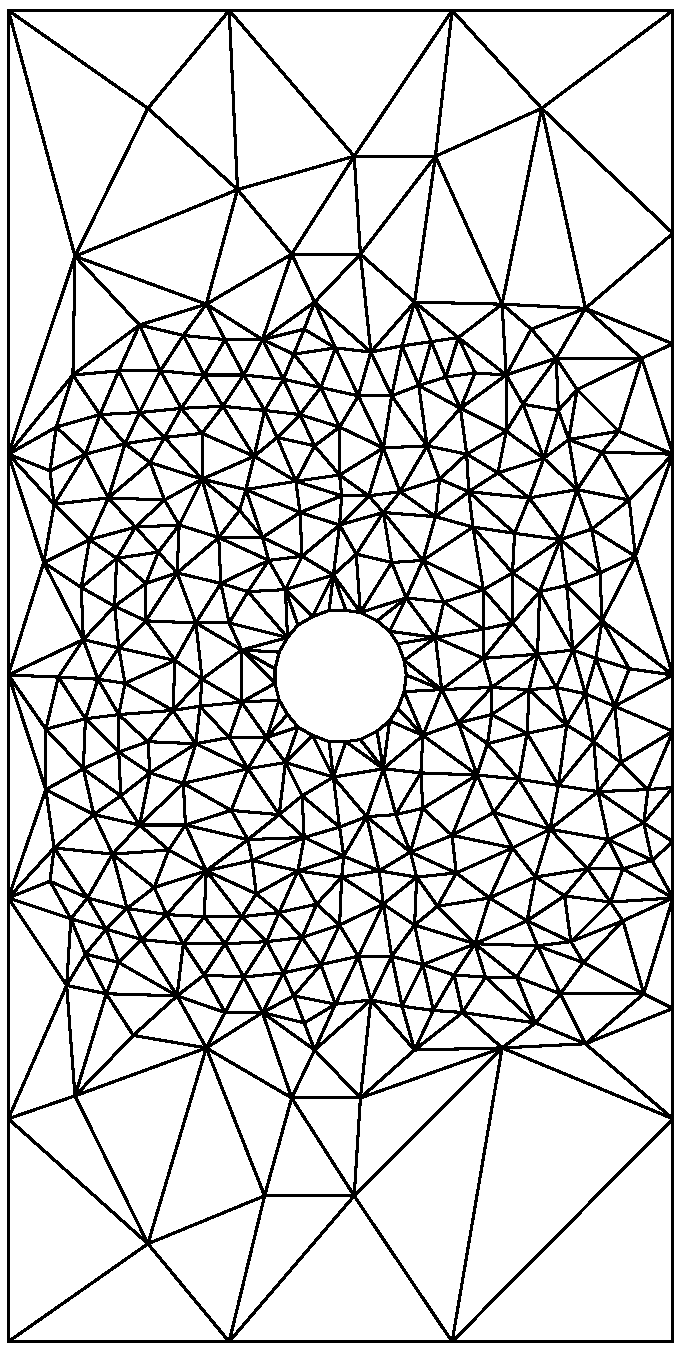
\includegraphics[width=\w]{../plots/mesh6ele_u.pdf}
\caption{Sample Refinement process using horizonal component of velocity as the error indicator.}   \label{fig:refine_u1}
\end{figure}

\setcounter{subfigure}{0}
\begin{figure}[h]
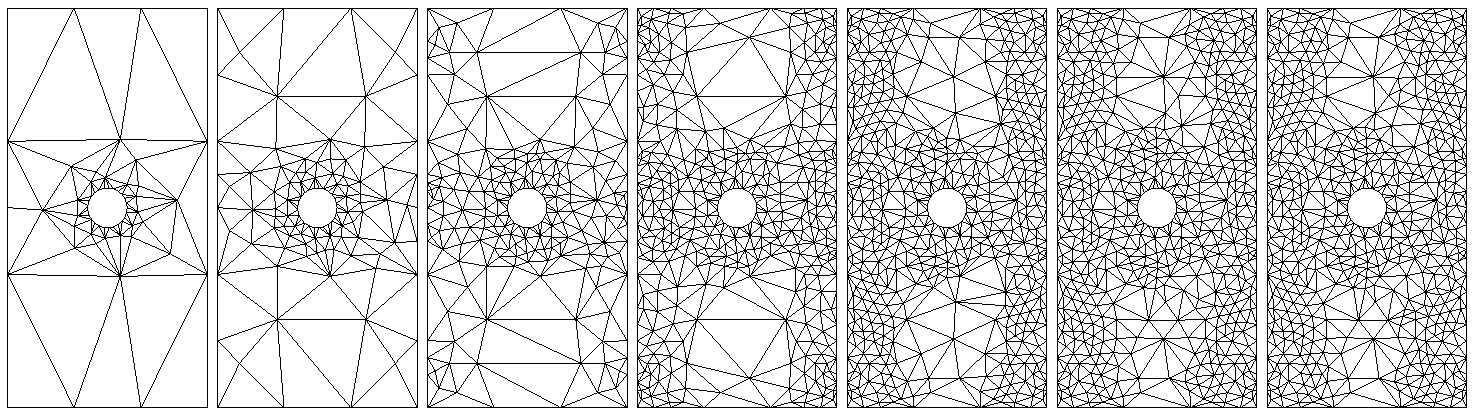
\includegraphics[height=\h]{../plots/v_1_row.pdf}
%\noindent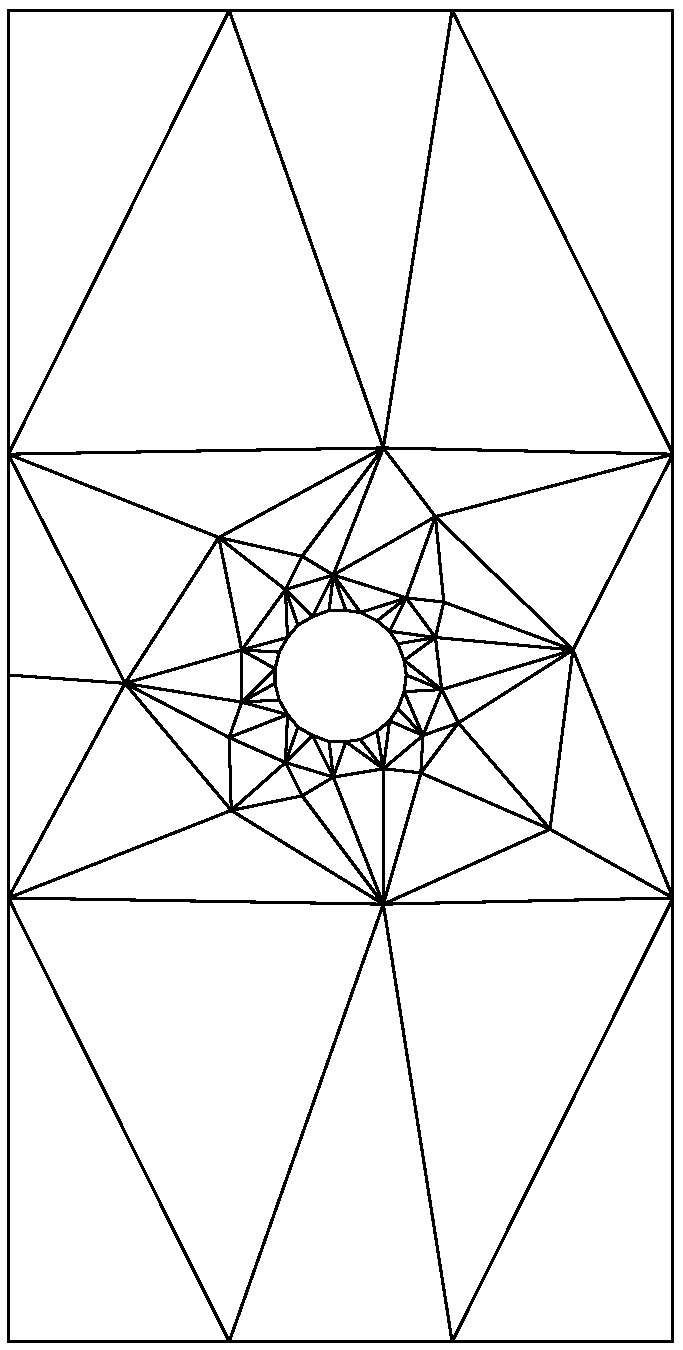
\includegraphics[width=\w]{../plots/mesh1ele_p.pdf}
%\noindent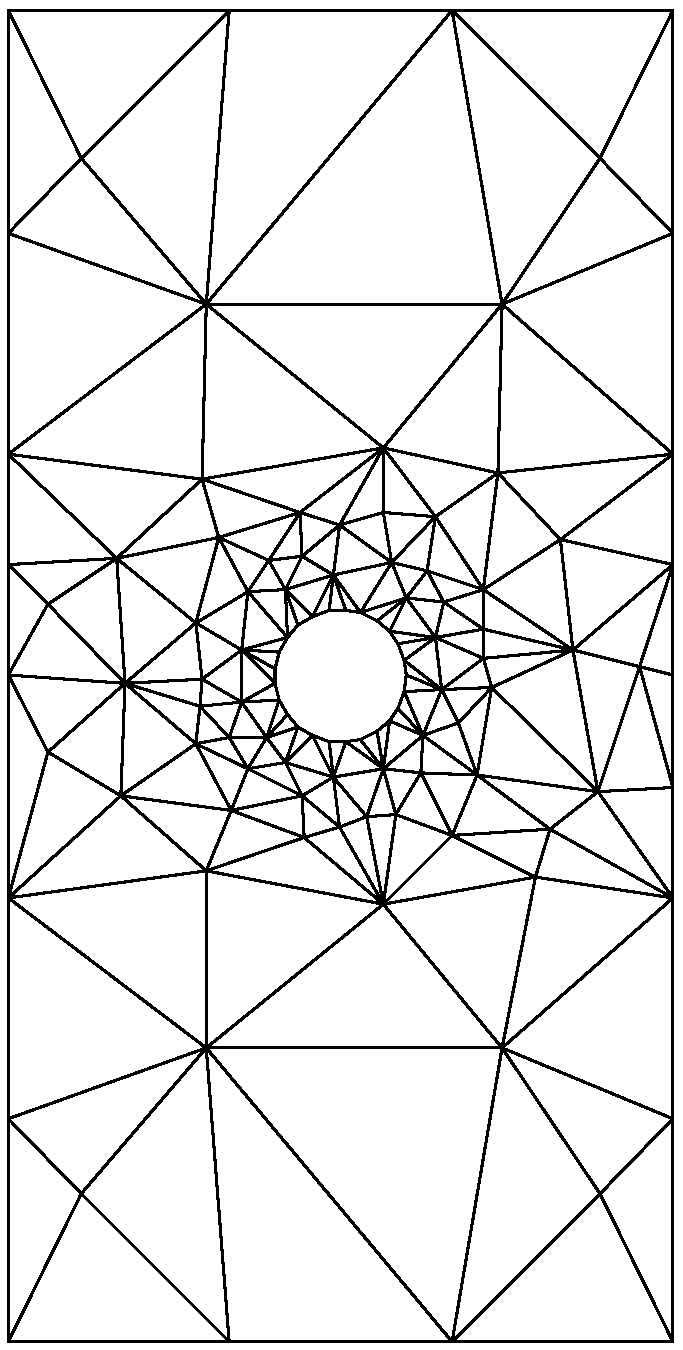
\includegraphics[width=\w]{../plots/mesh2ele_v.pdf}
%\noindent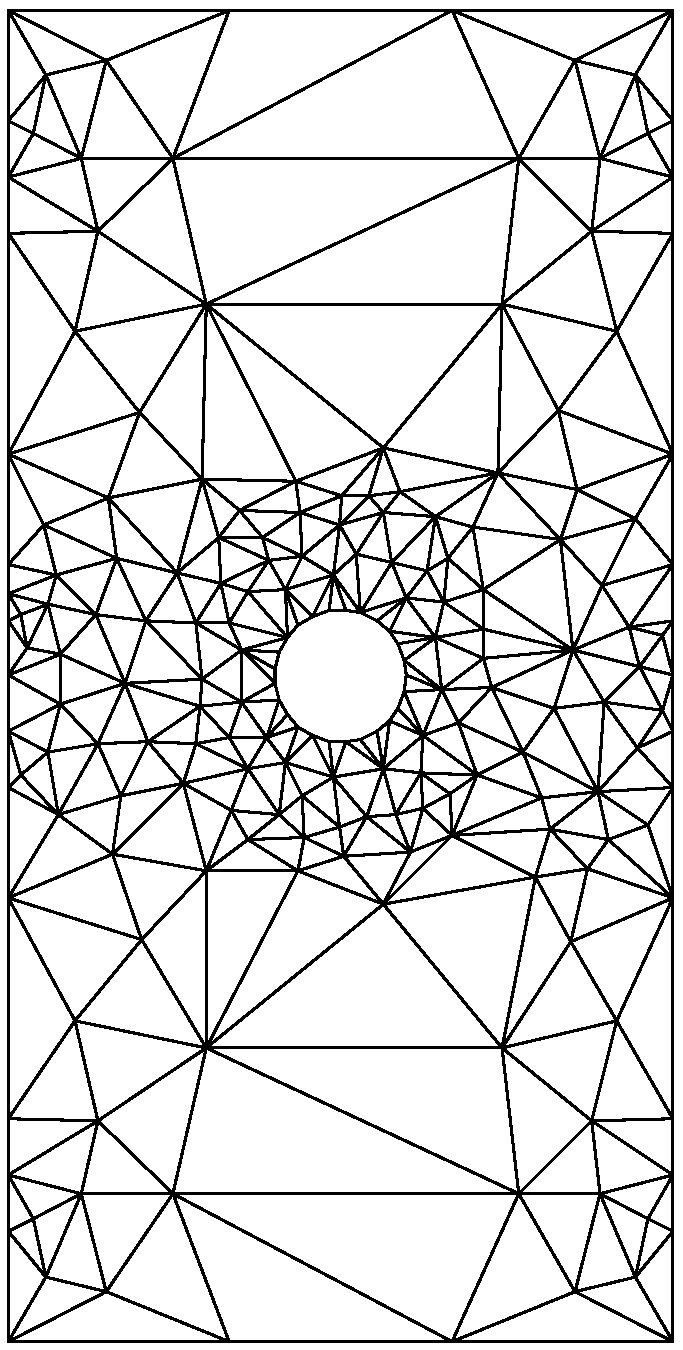
\includegraphics[width=\w]{../plots/mesh3ele_v.pdf}
%\noindent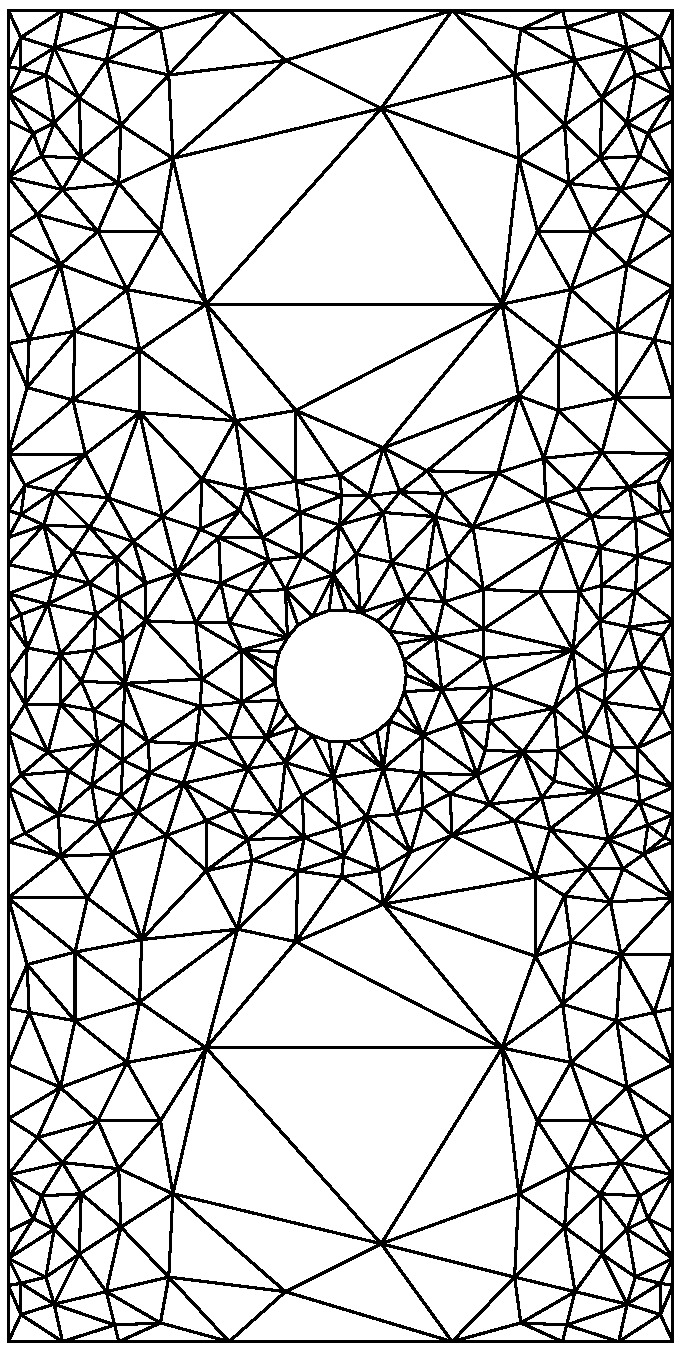
\includegraphics[width=\w]{../plots/mesh4ele_v.pdf}
%\noindent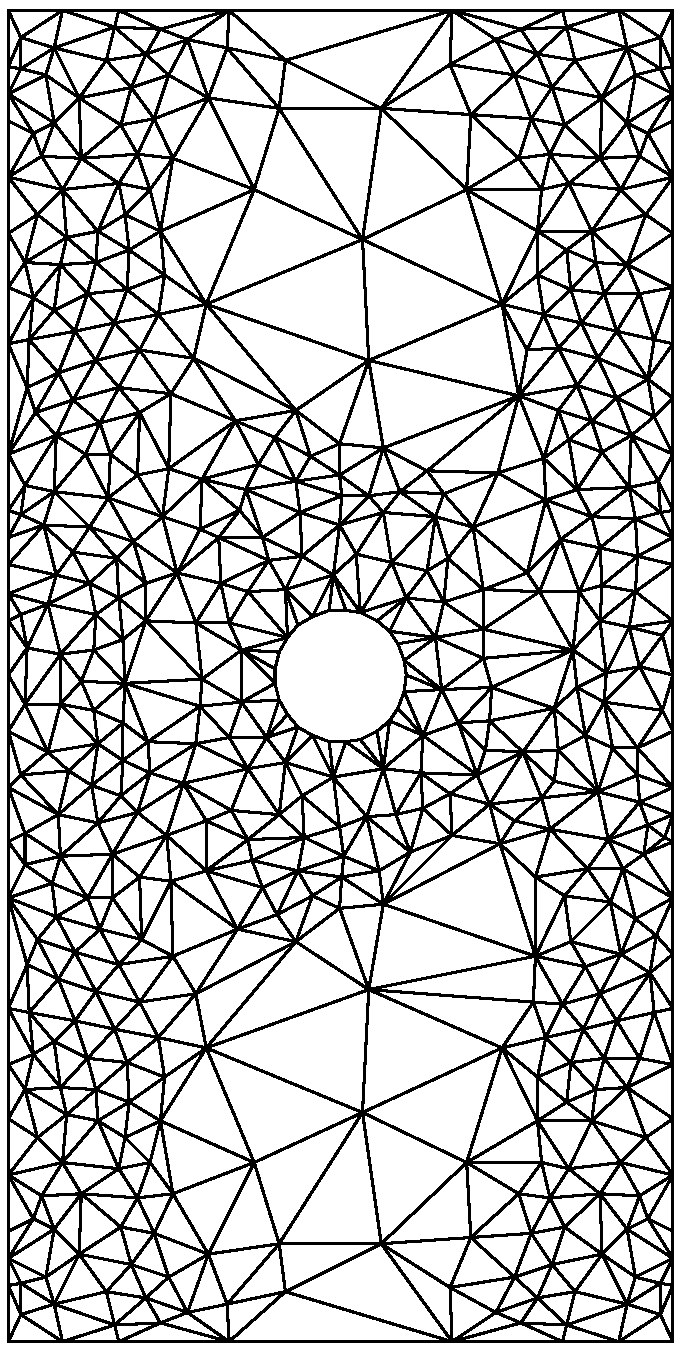
\includegraphics[width=\w]{../plots/mesh5ele_v.pdf}
%\noindent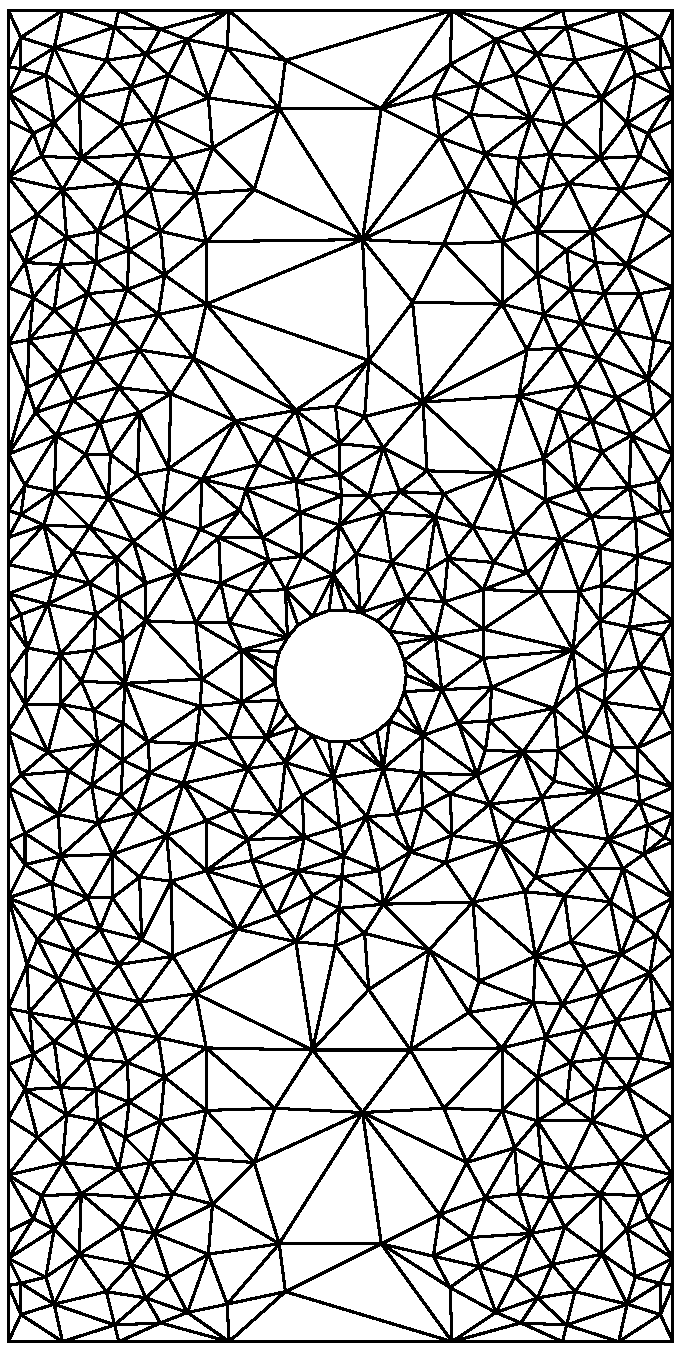
\includegraphics[width=\w]{../plots/mesh6ele_v.pdf}
%\noindent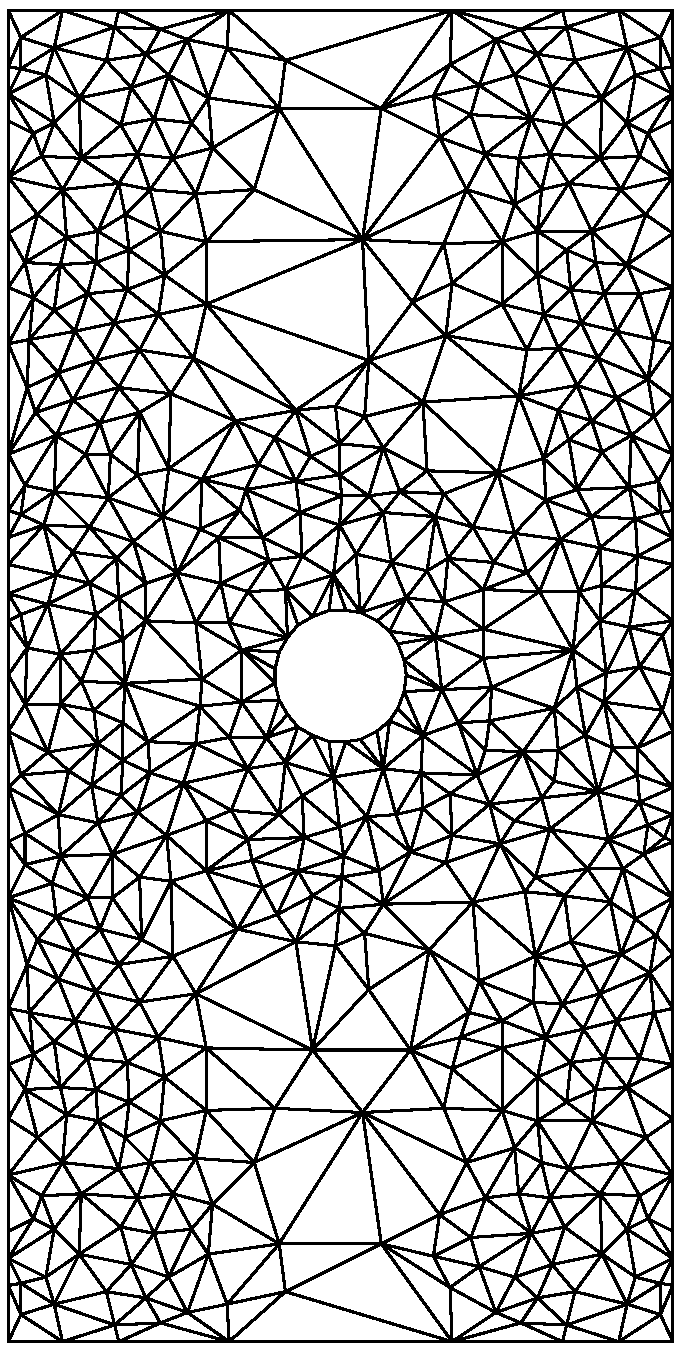
\includegraphics[width=\w]{../plots/mesh7ele_v.pdf}
\caption{Sample Refinement process with one cylinder using vertical component of velocity as the error indicator.}   \label{fig:refine_v1}
\end{figure}

\setcounter{subfigure}{0}
\begin{figure}[h]
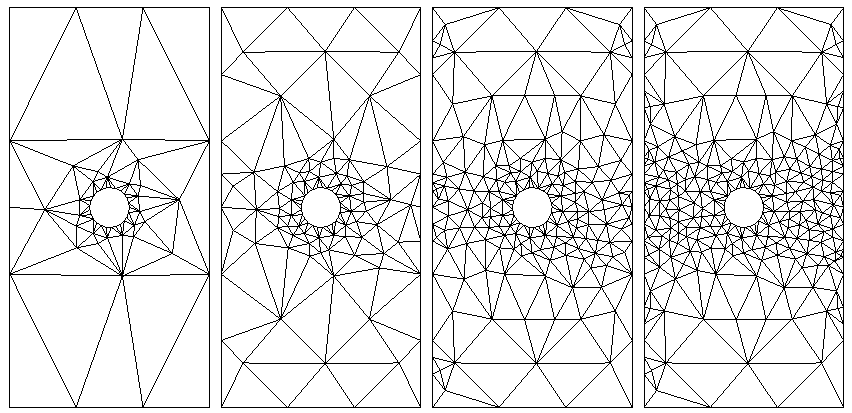
\includegraphics[height=\h]{../plots/p_1_row.pdf}
%\noindent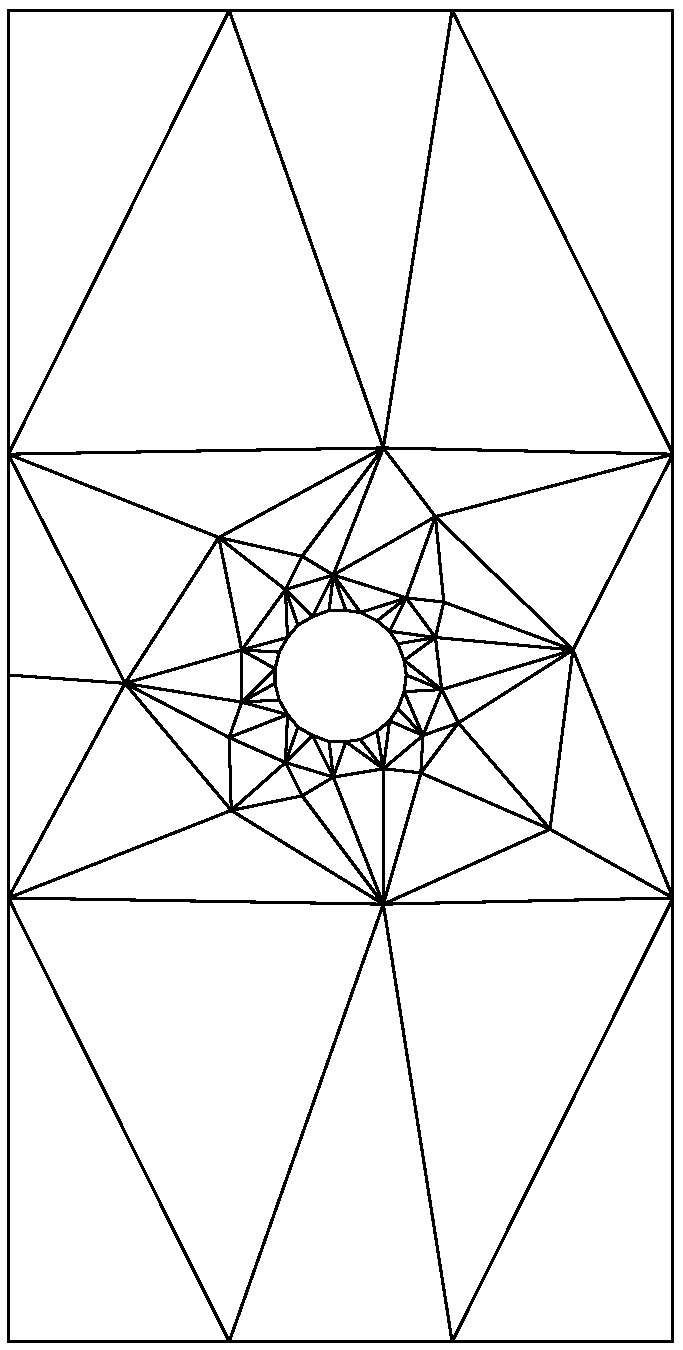
\includegraphics[width=\w]{../plots/mesh1ele_p.pdf}
%\noindent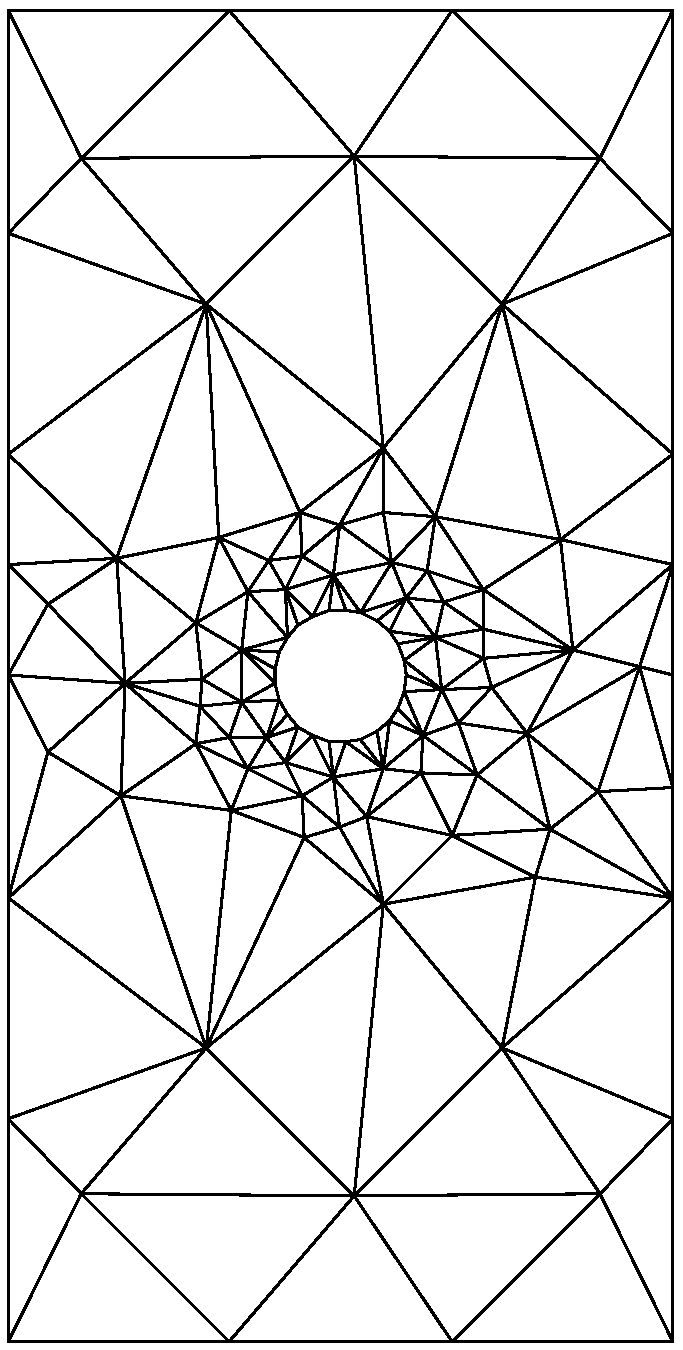
\includegraphics[width=\w]{../plots/mesh2ele_p.pdf}
%\noindent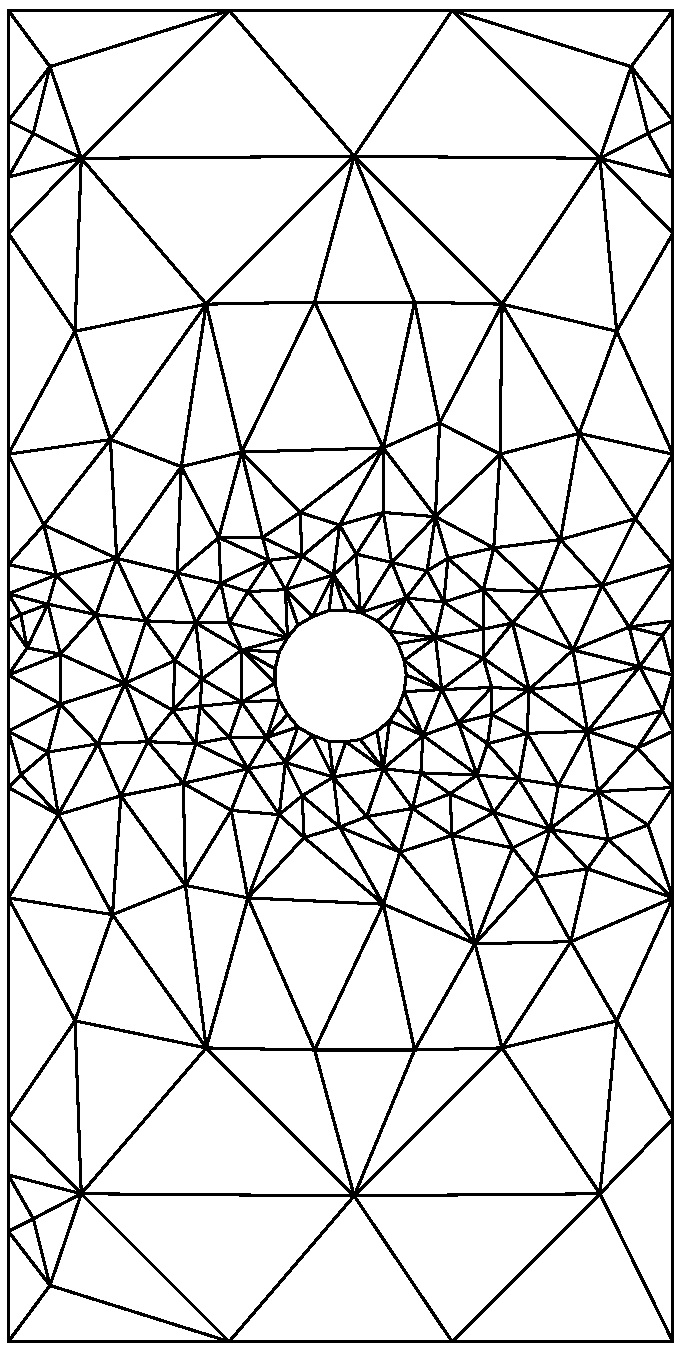
\includegraphics[width=\w]{../plots/mesh3ele_p.pdf}
%\noindent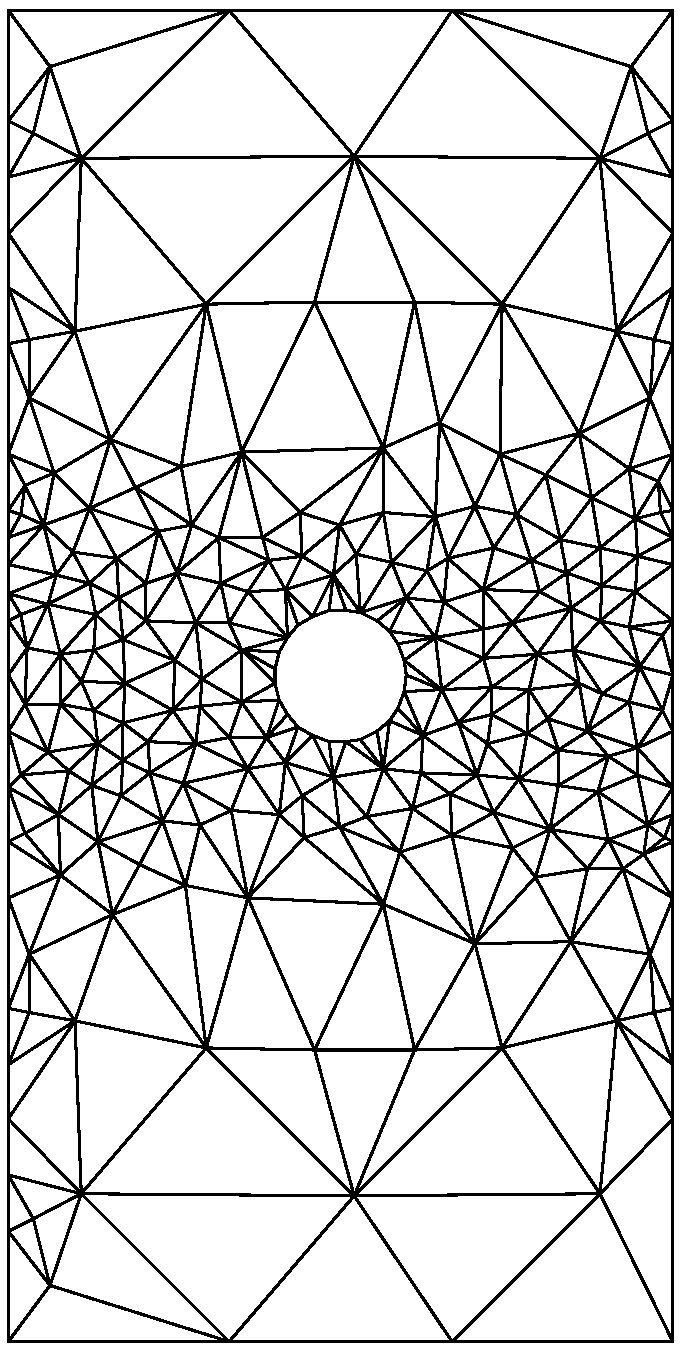
\includegraphics[width=\w]{../plots/mesh4ele_p.pdf}
\caption{Sample Refinement process using pressure as the error indicator.} \label{fig:refine_p1}
\end{figure} 

%%%%%%%%%%%%%%%%% 
%
%	5 holes
%
%%%%%%%%%%%%%%%%%
\break
\setcounter{subfigure}{0}
\begin{figure}[h]
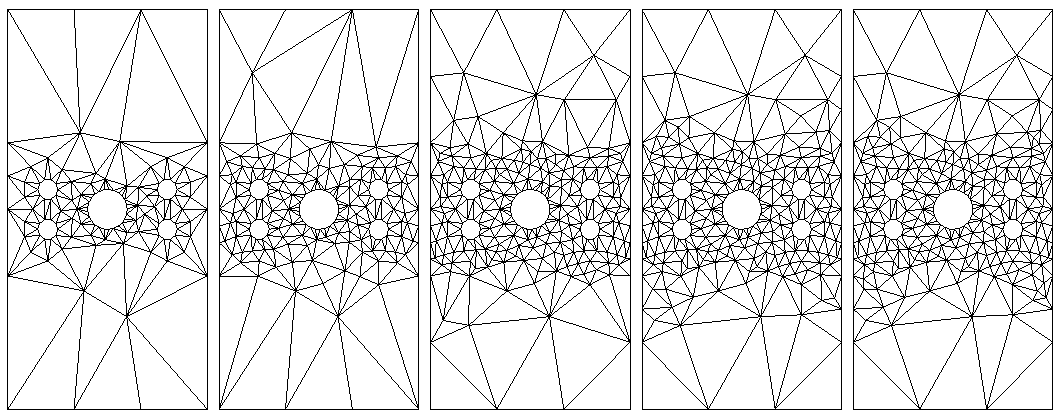
\includegraphics[height=\h]{../plots/u_5_row.pdf}
%\noindent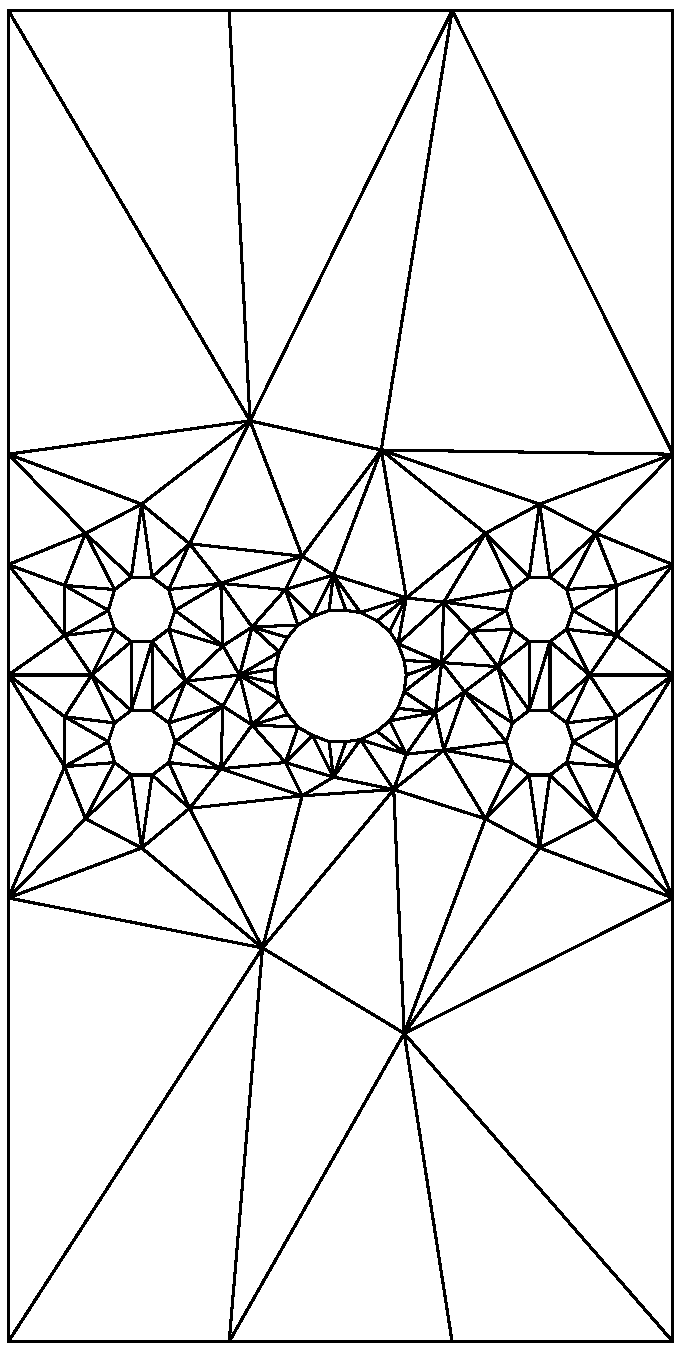
\includegraphics[width=\w]{../plots/mesh1ele_5.pdf}
%\noindent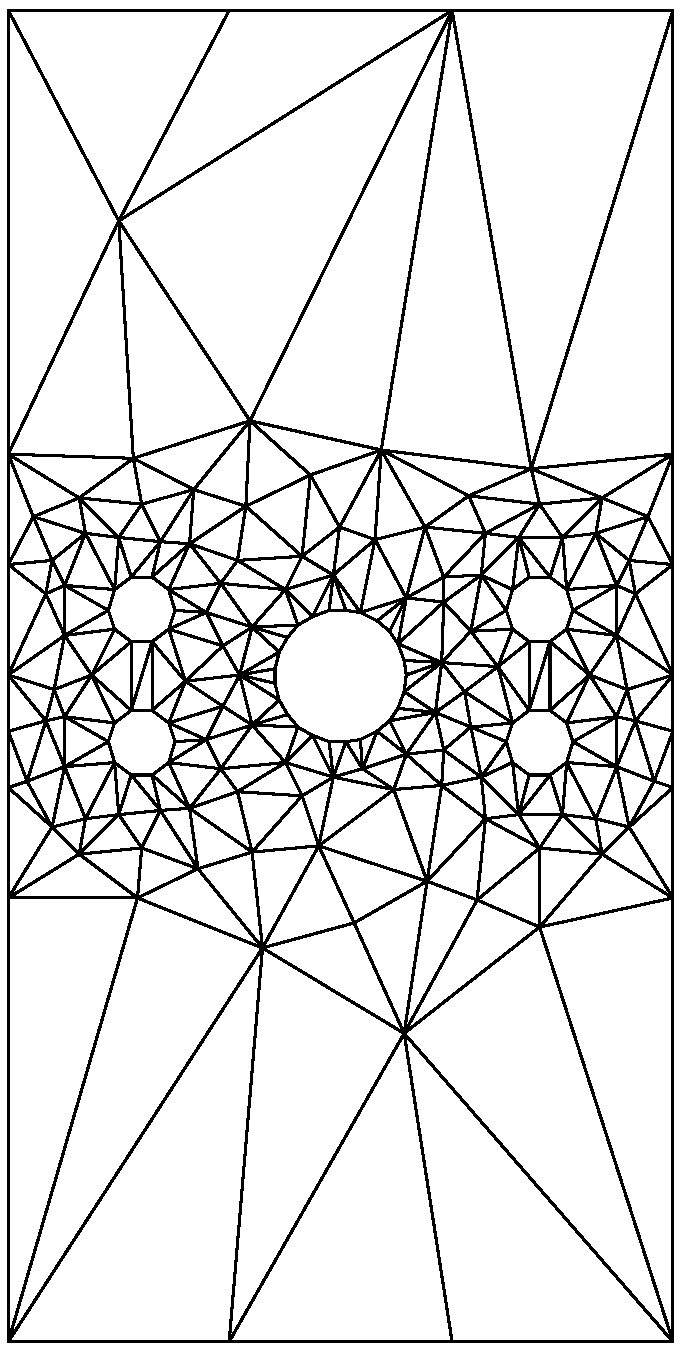
\includegraphics[width=\w]{../plots/mesh2ele_u5.pdf}
%\noindent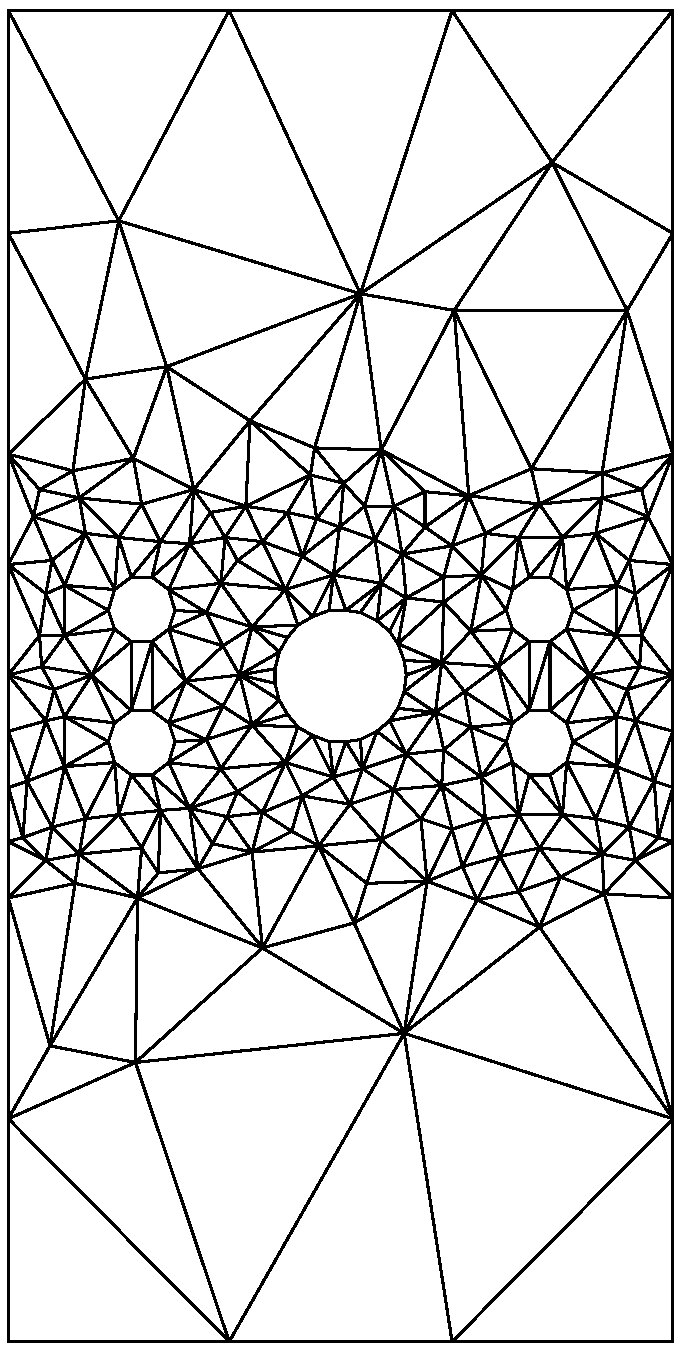
\includegraphics[width=\w]{../plots/mesh3ele_u5.pdf}
%\noindent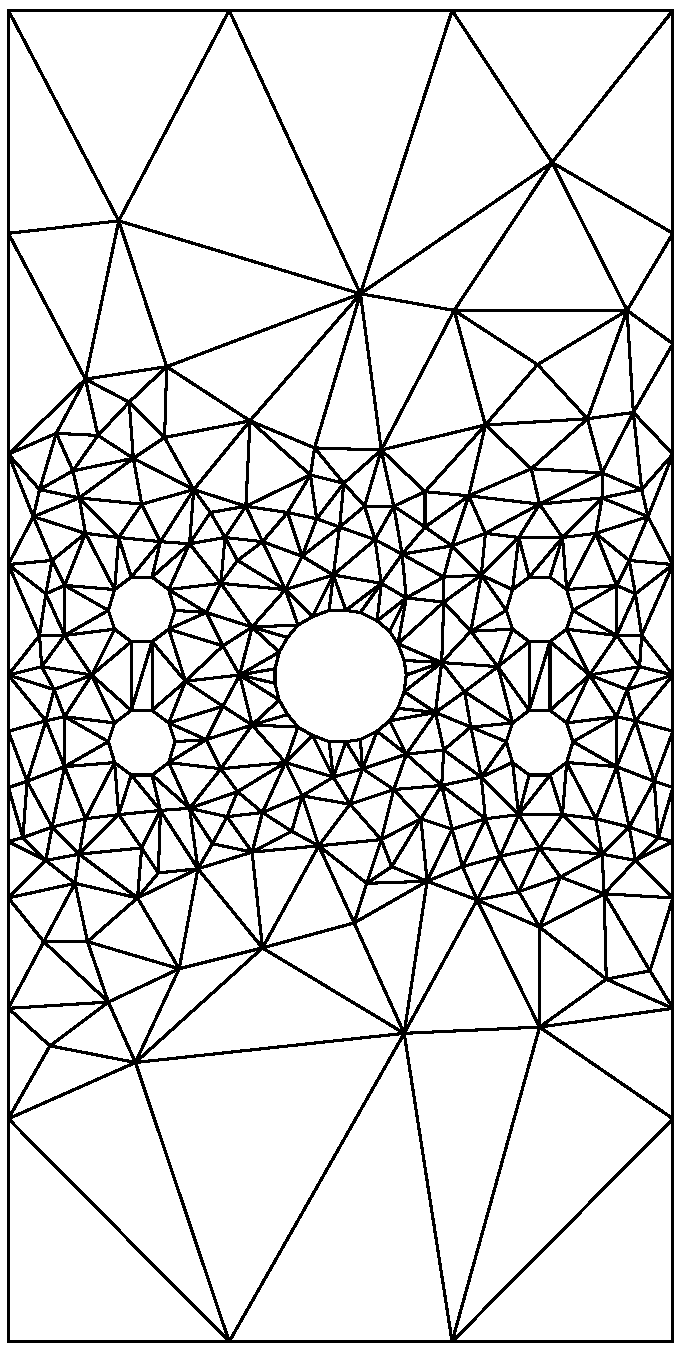
\includegraphics[width=\w]{../plots/mesh4ele_u5.pdf}
%\noindent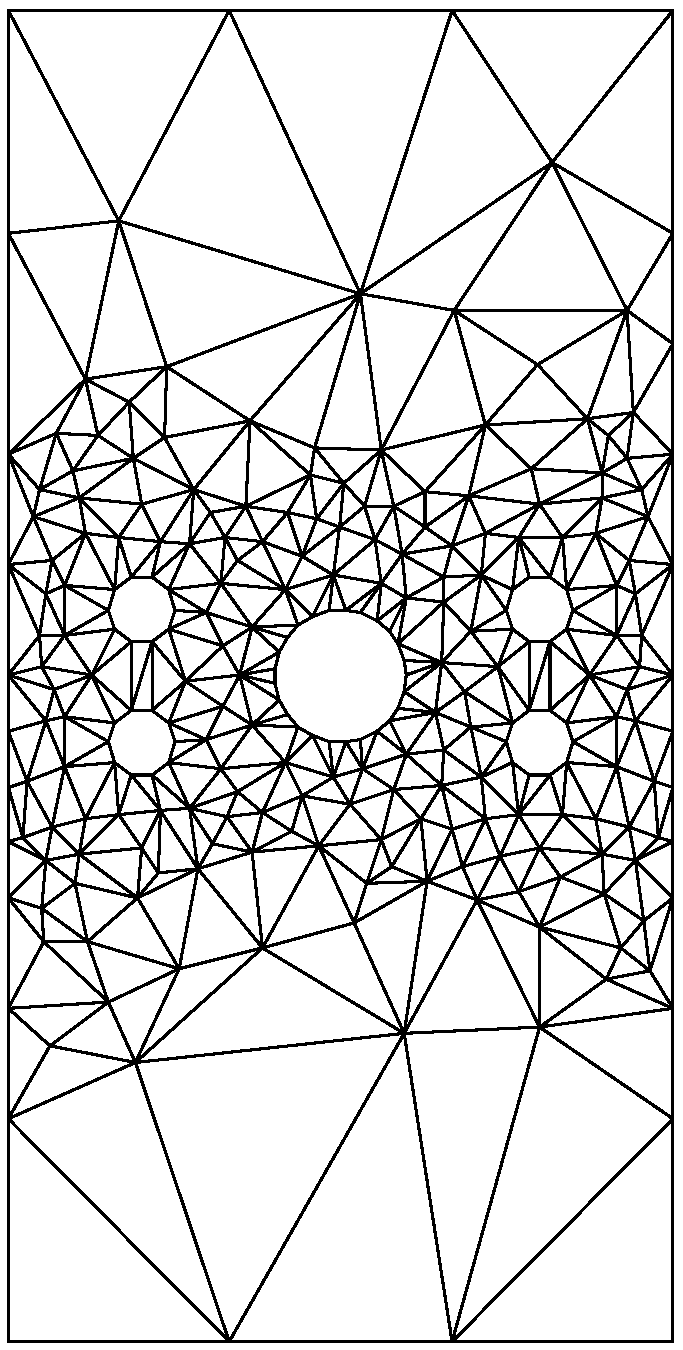
\includegraphics[width=\w]{../plots/mesh5ele_u5.pdf}
\caption{Sample Refinement process with 5 obstructions using horizonal component of velocity as the error indicator.}   
\end{figure}

\begin{figure}[h]
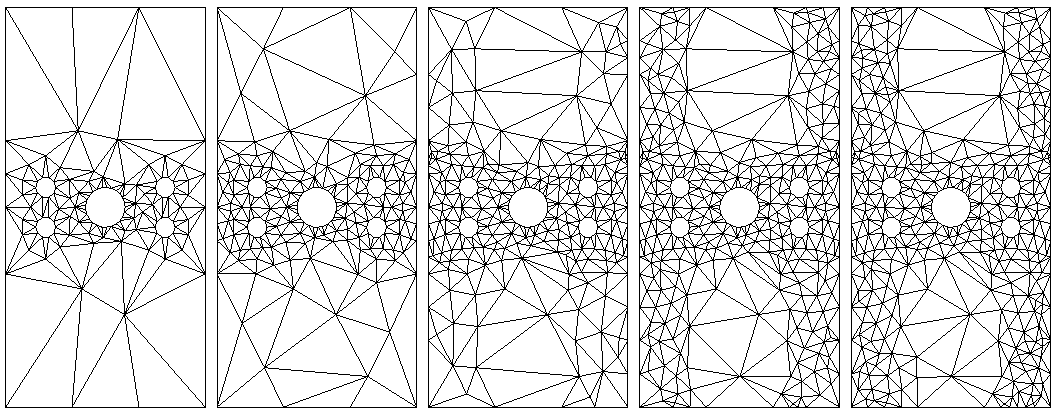
\includegraphics[height=\h]{../plots/v_5_row.pdf}
%\noindent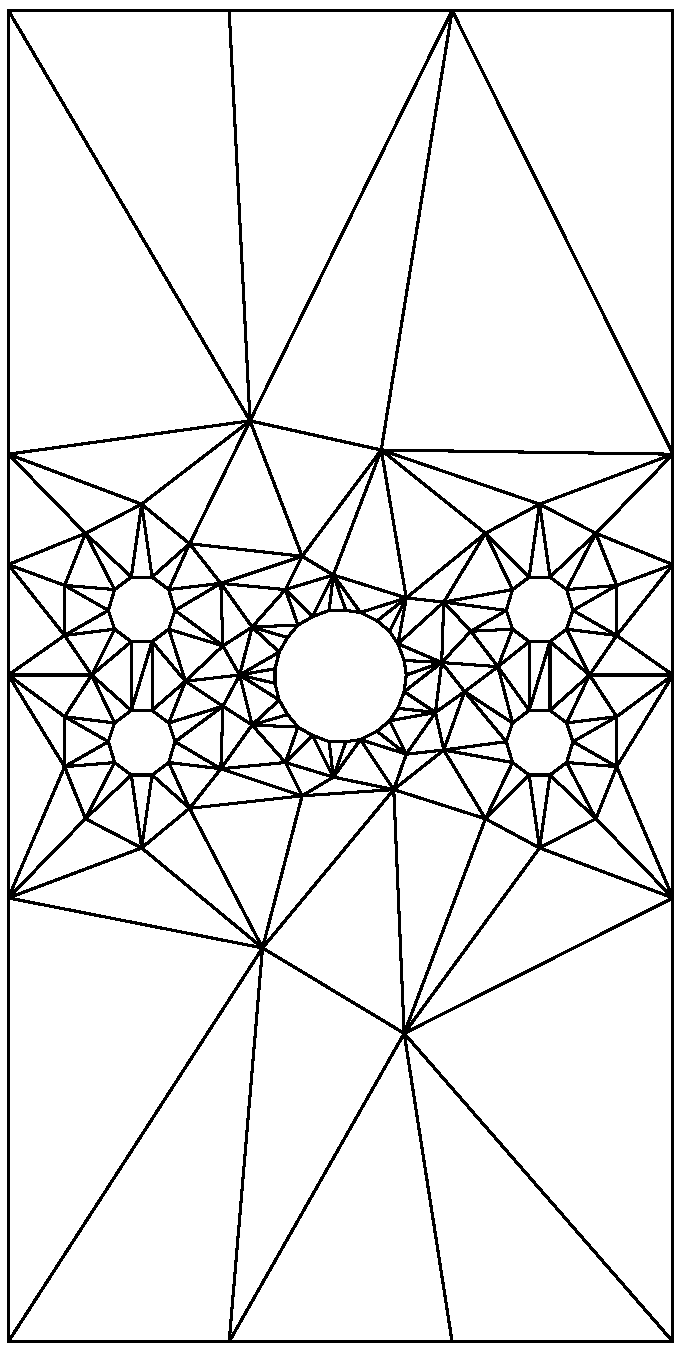
\includegraphics[width=\w]{../plots/mesh1ele_5.pdf}
%\noindent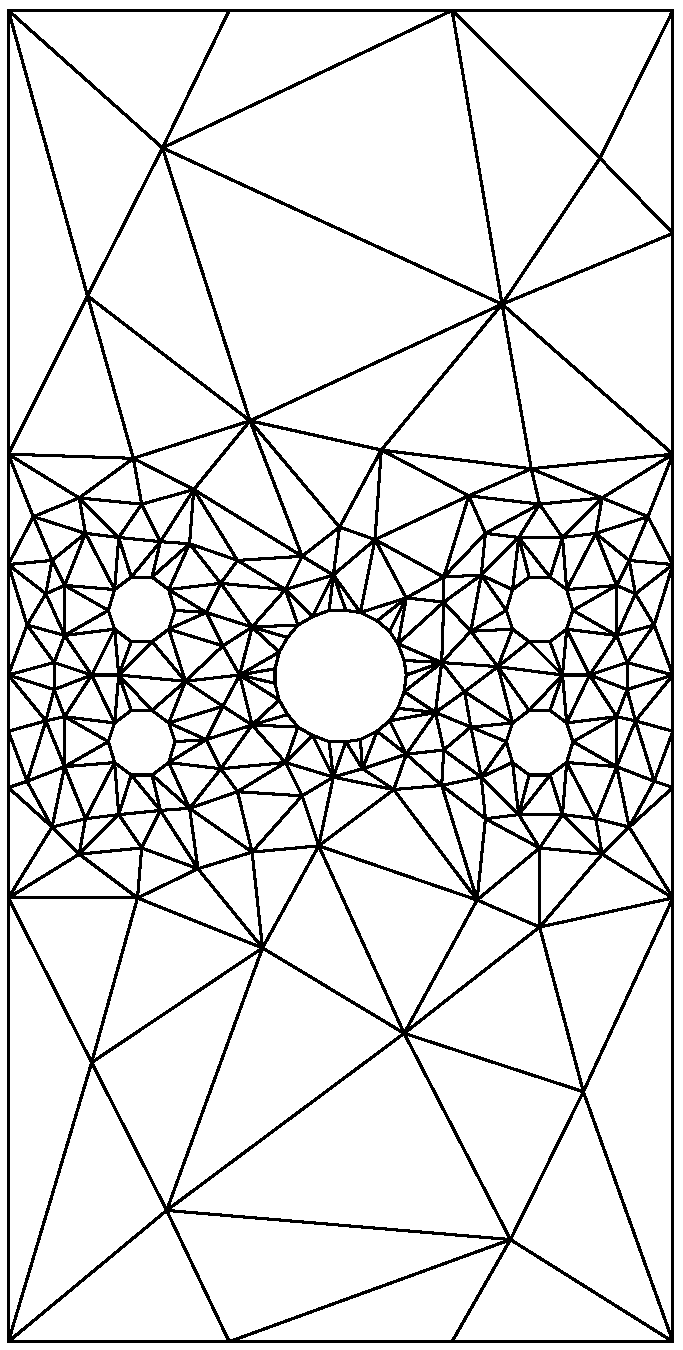
\includegraphics[width=\w]{../plots/mesh2ele_v5.pdf}
%\noindent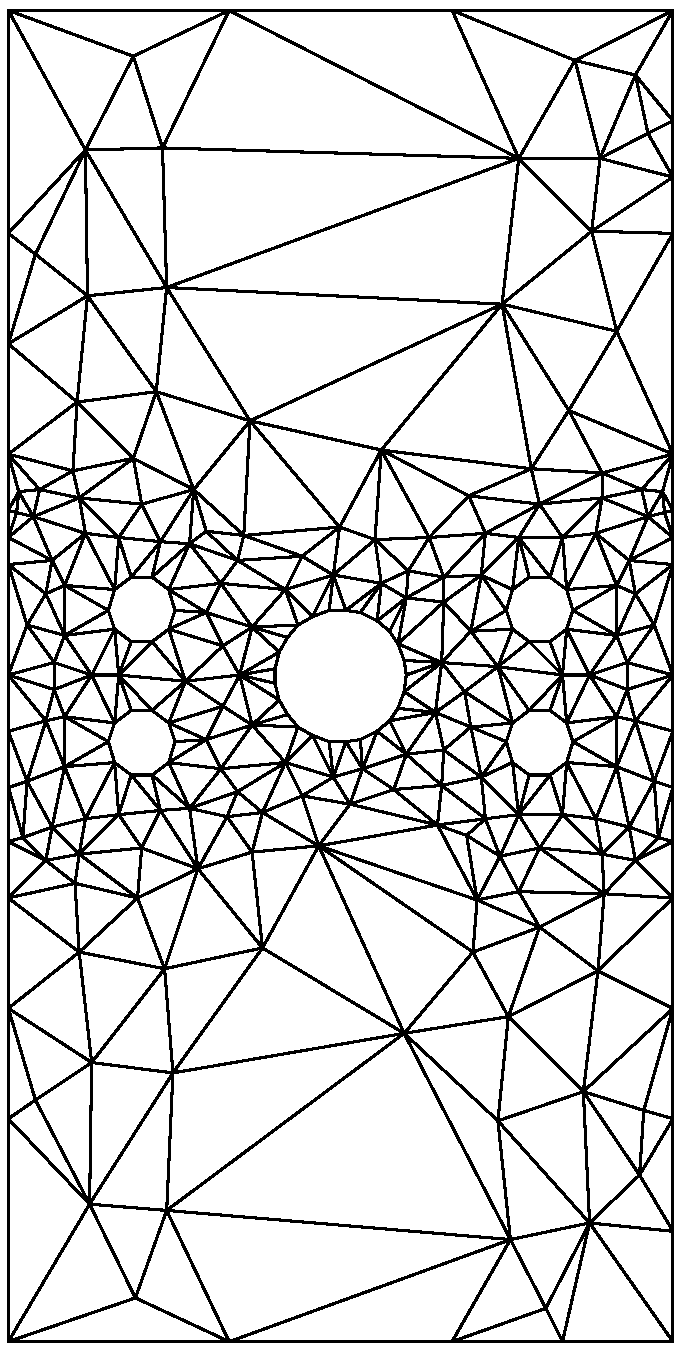
\includegraphics[width=\w]{../plots/mesh3ele_v5.pdf}
%\noindent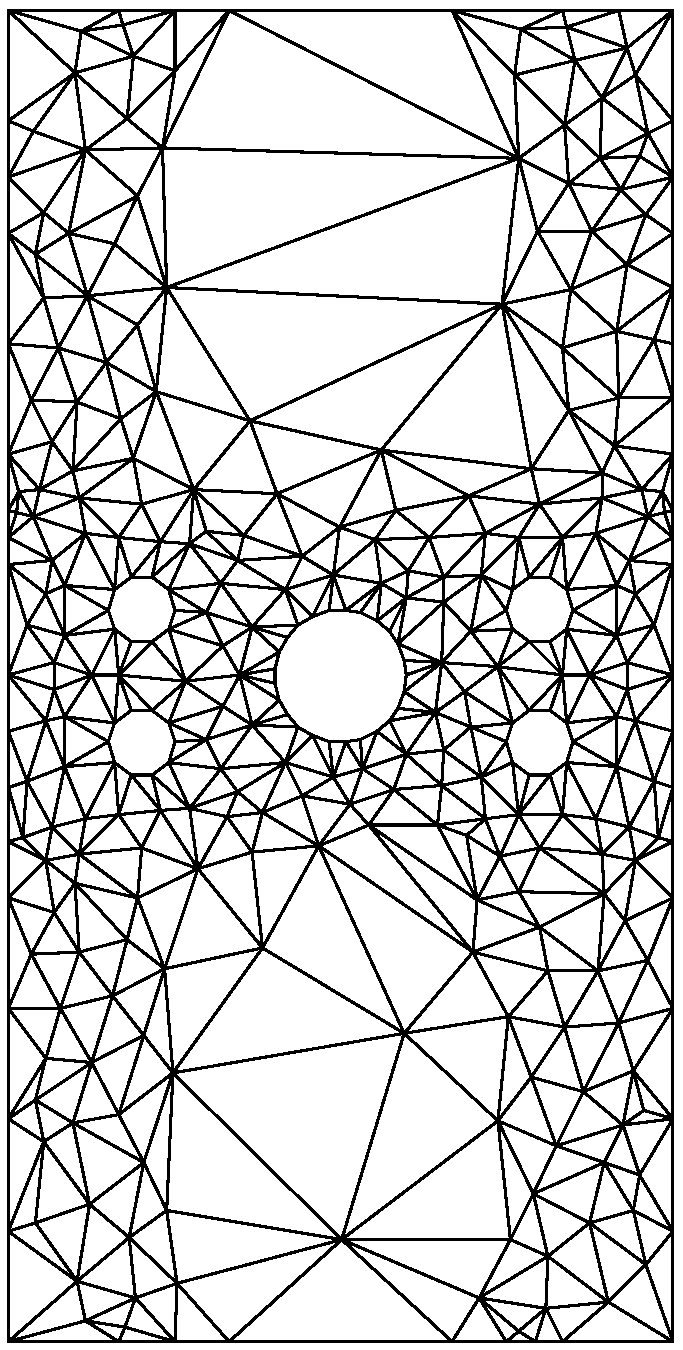
\includegraphics[width=\w]{../plots/mesh4ele_v5.pdf}
%\noindent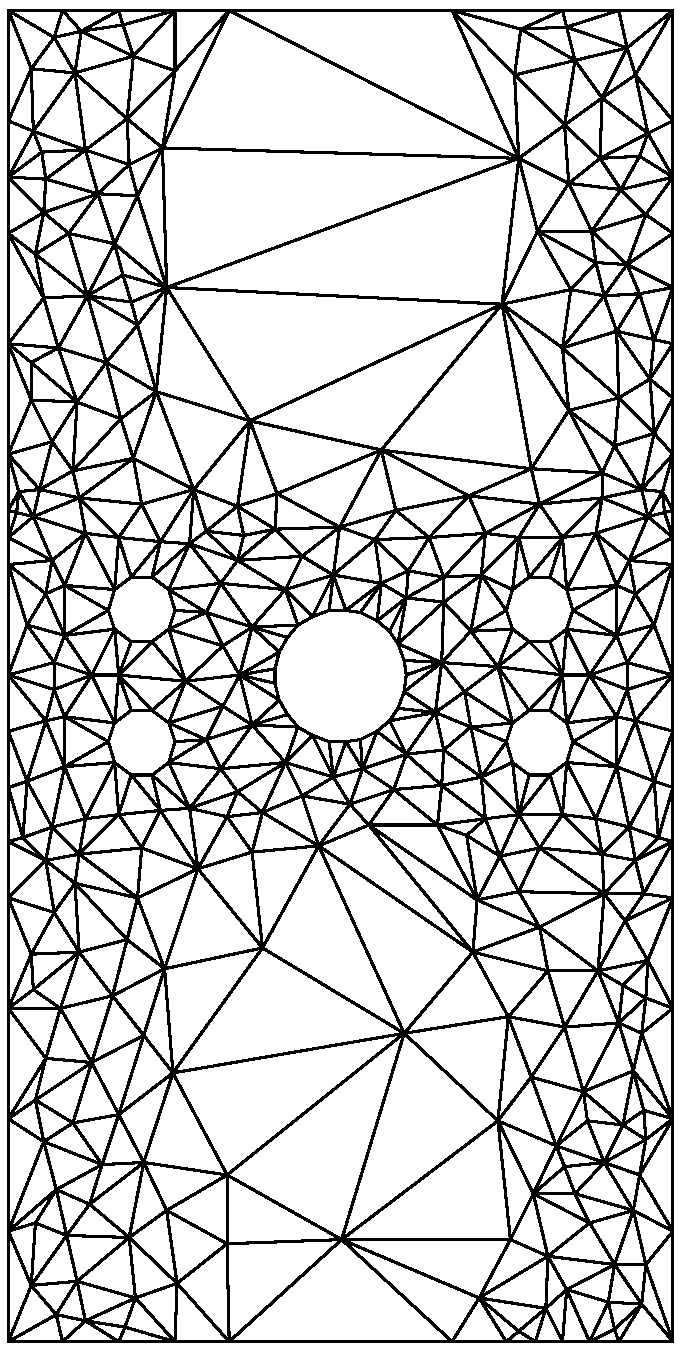
\includegraphics[width=\w]{../plots/mesh5ele_v5.pdf}
\caption{Sample Refinement process with 5 obstructions using vertical component of velocity as the error indicator.}   
\end{figure}

\begin{figure}[h]
\includegraphics[height=\h]{../plots/p_5_row.pdf}
%\noindent\includegraphics[width=\w]{../plots/mesh1ele_5.pdf}
%\noindent\includegraphics[width=\w]{../plots/mesh2ele_p5.pdf}
%\noindent\includegraphics[width=\w]{../plots/mesh3ele_p5.pdf}
%\noindent\includegraphics[width=\w]{../plots/mesh4ele_p5.pdf}
\caption{Sample Refinement process with 5 obstructions using pressure as the error indicator.}   
\end{figure}

%%%%%%%%%%%%%%%%% 
%
%		13 holes
%
%%%%%%%%%%%%%%%%%
\break
\begin{figure}[h]
\includegraphics[height=\h]{../plots/v_13_row.pdf}
%\noindent\includegraphics[width=\w]{../plots/mesh1ele_13.pdf}
%\noindent\includegraphics[width=\w]{../plots/mesh2ele_v13.pdf}
%\noindent\includegraphics[width=\w]{../plots/mesh3ele_v13.pdf}
%\noindent\includegraphics[width=\w]{../plots/mesh4ele_v13.pdf}
%\noindent\includegraphics[width=\w]{../plots/mesh5ele_v13.pdf}
\caption{Sample Refinement process with 13 obstructions using vertical component of velocity as the error indicator.}   
\end{figure}

\setcounter{subfigure}{0}
\begin{figure}[h]
\includegraphics[height=\h]{../plots/u_13_row.pdf}
%\noindent\includegraphics[width=\w]{../plots/mesh1ele_13.pdf}
%\noindent\includegraphics[width=\w]{../plots/mesh2ele_u13.pdf}
%\noindent\includegraphics[width=\w]{../plots/mesh3ele_u13.pdf}
%\noindent\includegraphics[width=\w]{../plots/mesh4ele_u13.pdf}
\caption{Sample Refinement process with 13 obstructions using horizonal component of velocity as the error indicator.}   
\end{figure}

\begin{figure}[h]
\includegraphics[height=\h]{../plots/p_13_row.pdf}
%\noindent\includegraphics[width=\w]{../plots/mesh1ele_13.pdf}
%\noindent\includegraphics[width=\w]{../plots/mesh2ele_p13.pdf}
%\noindent\includegraphics[width=\w]{../plots/mesh3ele_p13.pdf}
%\noindent\includegraphics[width=\w]{../plots/mesh4ele_p13.pdf}
\caption{Sample Refinement process with 13 obstructions using pressure as the error indicator.}   
\end{figure}

\newpage
%% ------------------------------------------------------------------------ %%
%
%  END ARTICLE
%
%% ------------------------------------------------------------------------ %%

\end{article}




























































































%% Enter Figures and Tables at here:

% When submitting articles through the GEMS system:
% COMMENT OUT ANY COMMANDS THAT INCLUDE GRAPHICS.

% Figure captions go below this illustration; Table captions above tables

% ONE-COLUMN figure/table, including eps graphics
%
% \begin{figure}
% \noindent\includegraphics[width=20pc]{adaptive.pdf}
% \caption{Caption text here}
% \end{figure}
%
% \begin{table}
% \caption{}
% \end{table}
%
% ---------------
% TWO-COLUMN figure/table
%
% \begin{figure*}
% \noindent\includegraphics[width=39pc]{samplefigure.pdf}
% \caption{Caption text here}
% \end{figure*}
%
% \begin{table*}
% \caption{Caption text here}
% \end{table*}
%
% see below for how to make landscape figures or tables

%%% End the article here:

\end{document}

%%%%%%%%%%%%%%%%%%%%%%%%%%%%%%%%%%%%%%%%%%%%%%%%%%%%%%%%%%%%%%%

More information and Advice:

%  SECTION HEADS

 ---------------
 Level 1 head

 Use the \section{} command to identify level 1 heads;
 type the appropriate head wording between the curly
 brackets, as shown below.

 Capitalize the first letter of each word (expect for
 prepositions, conjunctions, and articles that are
 three or fewer letters).

 Do not hyphenate level 1 heads. To break lines,
 type \protect\\ where you want the break to occur.
 AGU prefers the inverted triangle, breaking before
 prepositions, conjunctions, and articles, if possible.

An example:
\section{Level 1 Head: Introduction}

 ---------------
 Level 2 head

 Use the \subsection{} command to identify level 2 heads.

 Capitalize the first letter of each word (expect for
 prepositions, conjunctions, and articles that are
 three or fewer letters).

 Do not hyphenate level 1 heads. To break lines,
 type \protect\\ where you want the break to occur.
 AGU prefers the inverted triangle, breaking before
 prepositions, conjunctions, and articles, if possible.

\subsection{Level 2 Head} An example.

 ---------------
 Level 3 head

 Use the \subsubsection{} command to identify level 3 heads

 Capitalize only the first letter of the first word, acronyms,
 first letter of proper nouns, and first letter of first word
 after a colon.

 Hyphenation is permitted in level 3 heads, if needed.

\subsubsection{Level 3 Head} An example.

\subsubsubsection{Level 4 Head} An example.

%% ------------------------------------------------------------------------ %%
%
%  IN-TEXT LISTS
%
%% ------------------------------------------------------------------------ %%

% Do not use bulleted lists; enumerated lists are okay.
 \begin{enumerate}
 \item
 \item
 \item
 \end{enumerate}

%% ------------------------------------------------------------------------ %%
%
%  EQUATIONS
%
%% ------------------------------------------------------------------------ %%

% Single-line equations are centered.

 Math coded inside display math mode \[ ...\]
 will not be numbered e.g.:
 \[ x^2=y^2 + z^2\]

 Math coded inside \begin{equation} and \end{equation} will
 be automatically numbered e.g.:
 \begin{equation}
 x^2=y^2 + z^2
 \end{equation}

% IF YOU HAVE MULTI-LINE EQUATIONS, PLEASE
% BREAK THE EQUATIONS INTO TWO OR MORE LINES
% OF SINGLE COLUMN WIDTH (20 pc, 8.3 cm)
% using double backslashes (\\).

% To create multiline equations, use the
% \begin{eqnarray} and \end{eqnarray} environment
% as demonstrated below.
\begin{eqnarray}
  x_{1} & = & (x - x_{0}) \cos \Theta \nonumber \\
        && + (y - y_{0}) \sin \Theta  \nonumber \\
  y_{1} & = & -(x - x_{0}) \sin \Theta \nonumber \\
        && + (y - y_{0}) \cos \Theta.
\end{eqnarray}

If you don't want an equation number, use the star form:
\begin{eqnarray*}...\end{eqnarray*}

% Break each line at a sign of operation
% (+, -, etc.) if possible, with the sign of operation
% on the new line.

% Indent second and subsequent lines to align with
% the first character following the equal sign on the
% first line.

% Use an \hspace{} command to insert horizontal space
% into your equation if necessary. Place an appropriate
% unit of measure between the curly braces, e.g.
% \hspace{1in}; you may have to experiment to achieve
% the correct amount of space.

% There is another multiline equation environment:
% \begin{aguleftmath}...\end{aguleftmath}
% The equation is aligned left and the second line indents to
% the width of a paragraph indent (AGU style)


%% ------------------------------------------------------------------------ %%
%
%  EQUATION NUMBERING: COUNTER
%
%% ------------------------------------------------------------------------ %%

% You may change equation numbering by resetting
% the equation counter or by explicitly numbering
% an equation.

% To explicitly number an equation, type \eqnum{}
% (with the desired number between the brackets)
% after the \begin{equation} or \begin{eqnarray}
% command.  The \eqnum{} command will affect only
% the equation it appears with; LaTeX will number
% any equations appearing later in the manuscript
% according to the equation counter.
%
% To reset the equation counter, place the setcounter{equation}
% command in front of your equation(s).
%\setcounter{equation}{0}

% Set the equation counter to 0 if the next
% number needed is 1 or set it to 7 if the
% next number needed is 8, etc.
%
% The \setcounter{equation} command does affect
% equations appearing later in the manuscript.

% If you have a multiline equation that needs only
% one equation number, use a \nonumber command in
% front of the double backslashes (\\) as shown in
% the multiline equation above.



%%%%%%%%%%%%%%%%%%%%%%%%%%%%%%%%%%%%%%%%%%%%%%%%%%%%%%
%% Landscape figure and table examples
%
% ---------------
% Landscape (broadside) figure/table
% (These objects will not display properly in draft mode, use galley.)
%
% ONE-COLUMN landscape figure and table
%
% \begin{landscapefigure}
% \includegraphics[height=.75\mycolumnwidth,width=42pc]{samplefigure.pdf}
% \caption{Caption text here}
% \end{landscapefigure}
%
% \begin{landscapetable}
% \caption{Caption text here}
% \begin{tabular*}{\hsize}{@{\extracolsep{\fill}}lcccc}
% \tableline
% ....
% \tableline\\
% \multicolumn5l{(a) Algorithms from Numerical Recipes}\\
% \end{tabular*}
% \tablenotetext{}{}
% \tablecomments{}
% \end{landscapetable}
%
% FULL-PAGE landscape figures and tables
%
% \begin{figure*}[p]
% \begin{landscapefigure*}
% illustration here
% \caption{caption here}
% \end{landscapefigure*}
% \end{figure*}
%
% \begin{table}[p]
% \begin{landscapetable*}
% \caption{}
% \begin{tabular*}{\textheight}{@{\extracolsep{\fill}}lccrrrcrrr}
% ....
% \end{tabular*}
% \begin{tablenotes}
% ...
% \end{tablenotes}
% \end{landscapetable*}
% \end{table}
%
